%%%%%%%%%%%%%%%%%%%%%%%%%%%%%%%%%%%%%%%%%
% KOMA-Script Presentation
% LaTeX Template
% Version 1.1 (18/10/15)
%
% This template has been downloaded from:
% http://www.LaTeXTemplates.com
%
% Original Authors:
% Marius Hofert (marius.hofert@math.ethz.ch)
% Markus Kohm (komascript@gmx.info)
% Described in the PracTeX Journal, 2010, No. 2
%
% License:
% CC BY-NC-SA 3.0 (http://creativecommons.org/licenses/by-nc-sa/3.0/)
%
%%%%%%%%%%%%%%%%%%%%%%%%%%%%%%%%%%%%%%%%%

%%----------------------------------------------------------------------------------------
%	PACKAGES AND OTHER DOCUMENT CONFIGURATIONS
%%----------------------------------------------------------------------------------------

\documentclass{beamer} % KOMA script (article)

\linespread{1.12} % Increase line spacing for readability
%
%%------------------------------------------------
%% Colors
\usepackage{xcolor}	 % Required for custom colors
% Define a few colors for making text stand out within the presentation
\definecolor{mygreen}{RGB}{44,85,17}
\definecolor{myblue}{RGB}{34,31,217}
\definecolor{mybrown}{RGB}{194,164,113}
\definecolor{myred}{RGB}{255,66,56}
% Use these colors within the presentation by enclosing text in the commands below
\newcommand*{\mygreen}[1]{\textcolor{mygreen}{#1}}
\newcommand*{\myblue}[1]{\textcolor{myblue}{#1}}
\newcommand*{\mybrown}[1]{\textcolor{mybrown}{#1}}
\newcommand*{\myred}[1]{\textcolor{myred}{#1}}
%%------------------------------------------------
%
%%------------------------------------------------
%% Margins
\usepackage{geometry}
%%------------------------------------------------
%
%%------------------------------------------------
%% Fonts
\usepackage[T1]{fontenc}	 % For correct hyphenation and T1 encoding
\usepackage{lmodern} % Default font: latin modern font
\usepackage						{subfigure}
%\usepackage{fourier} % Alternative font: utopia
%\usepackage{charter} % Alternative font: low-resolution roman font
\renewcommand{\familydefault}{\sfdefault} % Sans serif - this may need to be commented to see the alternative fonts
%%------------------------------------------------
%
%%------------------------------------------------
% Various required packages
\usepackage{eso-pic,picture}
\usepackage{anyfontsize}
\usepackage		[version=4]		{mhchem}
\usepackage						{multirow}
%\usepackage{amsthm} % Required for theorem environments
%\usepackage{bm} % Required for bold math symbols (used in the footer of the slides)
\usepackage{graphicx} % Required for including images in figures
\usepackage{tikz} % Required for colored boxes
\usepackage{booktabs} % Required for horizontal rules in tables
\usepackage{multicol} % Required for creating multiple columns in slides
\usepackage{lastpage} % For printing the total number of pages at the bottom of each slide
\usepackage[english]{babel} % Document language - required for customizing section titles
\usepackage{microtype} % Better typography
\usepackage{tocstyle} % Required for customizing the table of contents
%%------------------------------------------------
%
%%------------------------------------------------
% Slide layout configuration
%\usepackage{scrpage2} % Required for customization of the header and footer
%\pagestyle{scrheadings} % Activates the pagestyle from scrpage2 for custom headers and footers
%\clearscrheadfoot % Remove the default header and footer
%\setkomafont{pageheadfoot}{\normalfont\color{black}\sffamily} % Font settings for the header and footer
%
%% Sets vertical centering of slide contents with increased space between paragraphs/lists
%%\makeatletter
%%\renewcommand*{\@textbottom}{\vskip \z@ \@plus 1fil}
%%\newcommand*{\@texttop}{\vskip \z@ \@plus .5fil}
%%\addtolength{\parskip}{\z@\@plus .25fil}
%%\makeatother
%
% Remove page numbers and the dots leading to them from the outline slide
\makeatletter
\newtocstyle[noonewithdot]{nodotnopagenumber}{\settocfeature{pagenumberbox}{\@gobble}}
\makeatother
\usetocstyle{nodotnopagenumber}
%
%\AtBeginDocument{\renewcaptionname{english}{\contentsname}{\Large Outline}} % Change the name of the table of contents
%%------------------------------------------------
%
%%------------------------------------------------
%% Header configuration - if you don't want a header remove this block
%\ihead{
%\hspace{-2mm}
%\begin{tikzpicture}[remember picture,overlay]
%\node [xshift=\paperwidth/2,yshift=-\headheight] (mybar) at (current page.north west)[rectangle,fill,inner sep=0pt,minimum width=\paperwidth,minimum height=2\headheight,top color=mygreen!64,bottom color=mygreen]{}; % Colored bar
%\node[below of=mybar,yshift=3.3mm,rectangle,shade,inner sep=0pt,minimum width=128mm,minimum height =1.5mm,top color=black!50,bottom color=white]{}; % Shadow under the colored bar
%shadow
%\end{tikzpicture}
%\color{white}\runninghead} % Header text defined by the \runninghead command below and colored white for contrast
%%------------------------------------------------
%
%%------------------------------------------------
%% Footer configuration
%\setlength{\footheight}{1cm} % Height of the footer
%%\addtokomafont{pagefoot}{\footnotesize} % Small font size for the footnote
%%
%%\ifoot{% Left side
%%\hspace{-2mm}
%%\begin{tikzpicture}[remember picture,overlay]
%%\node [xshift=\paperwidth/2,yshift=\footheight] at (current page.south west)[rectangle,fill,inner sep=0pt,minimum width=\paperwidth,minimum height=3pt,top color=mygreen,bottom color=mygreen]{}; % Green bar
%%\end{tikzpicture}
%%\myauthor\ \raisebox{0.2mm}{$\bm{\vert}$}\ \myuni % Left side text
%}
%\setbeamertemplate{footline}[page number]
%\beamertemplatenavigationsymbolsempty
\mode<presentation> {
%  \usetheme{Ilmenau}%
\usecolortheme{beaver}
%\usefonttheme{professionalfonts}
%\useinnertheme{circles}
%\useoutertheme{split}
%\setbeamercolor{title}{fg=black}
\setbeamertemplate{navigation symbols}{}
\setbeamercovered{transparent}
\definecolor{mygreen}{RGB}{44,85,17}
\setbeamercolor{frametitle}{fg=mygreen}
\setbeamertemplate{footline}[frame number]
%\setbeamercolor*{section in head/foot}{fg=rudi,bg=white}
%\setbeamercolor*{subsection in head/foot}{fg=rudi,bg=black}
\setbeamercolor{structure}{fg=mygreen}
}

%%------------------------------------------------
%% Theorem style
%\newtheoremstyle{mythmstyle} % Defines a new theorem style used in this template
%{0.5em} % Space above
%{0.5em} % Space below
%{} % Body font
%{} % Indent amount
%{\sffamily\bfseries} % Head font
%{} % Punctuation after head
%{\newline} % Space after head
%{\thmname{#1}\ \thmnote{(#3)}} % Head spec
%	
%\theoremstyle{mythmstyle} % Change the default style of the theorem to the one defined above
%\newtheorem{theorem}{Theorem}[section] % Label for theorems
%\newtheorem{remark}[theorem]{Remark} % Label for remarks
%\newtheorem{algorithm}[theorem]{Algorithm} % Label for algorithms
%\makeatletter % Correct qed adjustment
%%------------------------------------------------
%
%%------------------------------------------------
% The code for the box which can be used to highlight an element of a slide (such as a theorem)
%\newcommand*{\mybox}[2]{ % The box takes two arguments: width and content
%\par\noindent
%\begin{tikzpicture}[mynodestyle/.style={rectangle,draw=mygreen,thick,inner sep=2mm,text justified,top color=white,bottom color=white,above}]\node[mynodestyle,at={(0.5*#1+2mm+0.4pt,0)}]{ % Box formatting
%\begin{minipage}[t]{#1}
%#2
%\end{minipage}
%};
%\end{tikzpicture}
%\par\vspace{-1.3em}}
%%------------------------------------------------
%
%%%----------------------------------------------------------------------------------------
%%	PRESENTATION INFORMATION
%%%----------------------------------------------------------------------------------------
%
\newcommand*{\mytitle}{Influence of ambient conditions on NOVAC BrO measurements\hspace{2.5cm}\textcolor{mygreen}{.}} % Title
%\newcommand*{\runninghead}{Running Head} % Running head displayed on almost all slides
\newcommand*{\myauthor}{Elsa Wilken$^1$, Florian Dinger$^{1,2}$, Simon Warnach$^{1,2}$, \\
Nicole Bobrowski$^{1,2}$, Ulrich Platt$^{1,2}$
\begin{flushright}
	
\end{flushright}} % Presenters name(s)
\newcommand*{\mydate}{\today} % Presentation date
\newcommand*{\myuni}{$^1$Heidelberg University --- Institute of Environmental Physics\\
	$^2$MPIC Mainz\hspace{7.4cm} \textcolor{white}{.}\\} % University or department

%%
%%%%----------------------------------------------------------------------------------------
%
\begin{document}
	
	\setcounter{framenumber}{0}
	
	%
	%%%----------------------------------------------------------------------------------------
	%%	TITLE SLIDE
	%%%----------------------------------------------------------------------------------------
	\begin{frame}
		
		
		% Title slide - you may have to tweak a few of the numbers if you wish to make changes to the layout
		\thispagestyle{empty} % No slide header and footer
		\begin{tikzpicture}[remember picture,overlay] % Background box
		\node [xshift=\paperwidth/2,yshift=\paperheight/1.7] at (current page.south west)[rectangle,fill,inner sep=0pt,minimum width=\paperwidth,minimum height=\paperheight/2.5,top color=mygreen,bottom color=mygreen]{}; % Change the height of the box, its colors and position on the page here
		\end{tikzpicture}
		% Text within the box
		\begin{flushright}
			\vspace{1cm}
			\color{white}\sffamily
			{\bfseries\Large\mytitle\par} % Title
			\vspace{0.8cm}
			\normalsize
			\myauthor\par % Author name
			\color{black}\sffamily
			\myuni % 
			\mydate\par % Date
			\vfill
		\end{flushright}
	\end{frame}
	
	
	%%----------------------------------------------------------------------------------------
	%	TABLE OF CONTENTS
	%%----------------------------------------------------------------------------------------
	%\begin{frame}
	
	%
	%\thispagestyle{empty} % No slide header and footer
	%
	%\small\tableofcontents % Change the font size and print the table of contents - it may be useful to shrink the font size further if the presentation is full of sections
	%% To exclude sections/subsections from the table of contents, put an asterisk after \(sub)section like so: \section*{Section Name}
	%
	%\end{frame}
	
	%%----------------------------------------------------------------------------------------
	%	PRESENTATION SLIDES
	%%----------------------------------------------------------------------------------------
	
\section{Motivation}
%\textit{Goal} Obtain Data about the volcanic emissions in real time in order to gain another quantity used in immanent risk assessment\\
%\item halogen sulfur ratio can be used as a proxy for volcanic processes\\
%\item Im vulkan sind die gase wie sulphur oder halogen gelöst im Magma. Es enstehen gasblasen, wenn der partiale Druck den umgebungsdruck übersteigt. Gas formation hört auf, wenn der partiale Druck der verbleibenden lösung im Magma den umgebungsdruck untersteigt. der partiale druck kann durch die Henry gesetz beschrieben werden.
%
%\fbox{\parbox{0.8\textwidth}{
%\begin{block}{Henry-Law}
%\begin{equation*}
%p = K_H\cdot c
%\end{equation*}
%\end{block}
%}}
%
%p: eqilibrium partial pressure; $K_H$ Henry konstant(T,chemical composition)\\
%pressure in magmatic chamber below volcano increases with depth. deswegen wird das gas bei einer bestimten tiefe
%abhängig von dem partialen Druck, der concentration im Magma und löslichkeit. Desweiteren wird rising zu einer erhöten gas formation führen. deshalb wird für jedes Gas der prozentuale Anteil mit der Tiefe sich ändern.
%Da sich die Abhängikeit aller Gase vom Druck unterscheidet kann aus dem verhältniss zwieer Gase rückschlüsse auf die Tiefe des magmas geschlossen wernden.
%Da gas leichter ist als magma steigt es schneller auf->
%solutible curve isnt yet avaliable.
%But one could observe at etna three month a higher ratio BrO/SO2
%\begin{frame}
%\frametitle{\color{mygreen}Motivation\\%\rule{_Breite_}{_Stärke_} %%andersrum ist's vertikal;)
%\color{mygreen}{\rule{0.8\textwidth}{2pt}}}
%\begin{enumerate}
%
%
%\item Im vulkan sind die gase wie sulphur oder halogen gelöst im Magma.
%\item Es enstehen gasblasen, wenn der partiale Druck den umgebungsdruck übersteigt. 
%\item Gas formation hört auf, wenn der partiale Druck der verbleibenden lösung im Magma den umgebungsdruck untersteigt.
%\item 
%\fbox{\parbox{2cm}{
%%\begin{block}{Henry-Law}
%\begin{equation*}
%p = K_H\cdot c
%\end{equation*}
%%\end{block}
%}}
%
%p: eqilibrium partial pressure; $K_H$ Henry konstant(T,chemical composition)\\
%\item pressure in magmatic chamber below volcano increases with depth. 
%\item deswegen wird das gas bei einer bestimten tiefe abhängig von dem partialen Druck, der concentration im Magma und löslichkeit. 
%\item Desweiteren wird rising zu einer erhöten gas formation führen. 
%\item deshalb wird für jedes Gas der prozentuale Anteil mit der Tiefe sich ändern.
%\item Da sich die Abhängikeit aller Gase vom Druck unterscheidet kann aus dem verhältniss zwieer Gase rückschlüsse auf die Tiefe des magmas geschlossen wernden.
%\item Da gas leichter ist als magma steigt es schneller auf->
%solutible curve isnt yet avaliable.
%\item But one could observe at etna three month a higher ratio BrO/SO2
%\end{enumerate}
%\end{frame}

%----------------------------------------------------------------------------------------\section{Motivation}
\setcounter{framenumber}{0}
%\begin{frame}
%\frametitle{\color{mygreen}Motivation\\%\rule{_Breite_}{_Stärke_} %%andersrum ist's vertikal;)
%\color{mygreen}{\rule{0.8\textwidth}{2pt}}}
%\begin{enumerate}
%
%\item The ratio of BrO and SO2 contains informations about its degassing source depth
%%\item Henry-Law  :     \fbox{\parbox{2cm}{
%%\begin{block}{Henry-Law}
%%\begin{equation*}
%%p = K_H\cdot c
%%\end{equation*}
%%\end{block}
%%}}
%
%\item Since the gas is less dense than the magma inside of a volcano, it will raise faster
%\item The ratio of BrO and SO2 is a proxy for the volcanic activity
%%\item One could observe at Etna three month prior to an eruption a higher ratio BrO/SO2
%\end{enumerate}
%\end{frame}


\begin{frame}
	\frametitle{\color{mygreen}Motivation for BrO measurements\\%\rule{_Breite_}{_Stärke_} %%andersrum ist's vertikal;)
		\color{mygreen}{\rule{0.8\textwidth}{2pt}}}
	\begin{multicols}{2}
		
		
		\begin{itemize}
			
			
			
			\item The ratio of BrO and SO$_2$ changes with degassing source depth
			%\item Remote sensing: BrO and SO$_2$
			\item The ratio of BrO and SO$_2$ is a proxy for the volcanic activity
			\item Change in BrO/SO$_2$ prior to eruption observed at Etna and Nevado del Ruiz
			
		\end{itemize}
		\begin{figure}
			\centering
			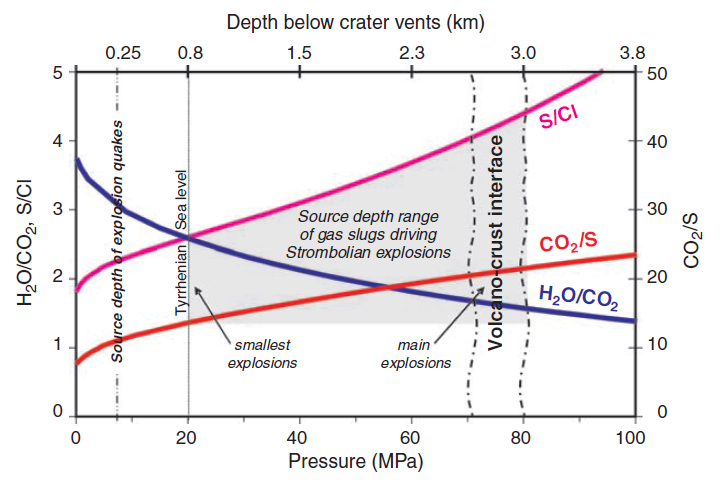
\includegraphics[width=1.2\linewidth]{../../Bilder/so2_bro}
			\label{fig:bro_so2}
		\end{figure}
		
	\end{multicols}
\end{frame}


%----------------------------------------------------------------------------------------\section{Motivation}





\subsection{Network for Observation of Volcanic and Atmospheric Change (NOVAC)}

%\textit{Initially} founded by European union. between 2005 and 2010
%Over 80 Instruments are installed at about 30 active volcanoes (most in south America, few in arfrica, europe)\\
%each volcano is typically monitored with two to four Novac stations.\\
%\textit{Location}: typically located 5-10 km downwind
%\textit{saved in} on servers at chalmers university sweden, uni Heidelberg, belgian Institute for space astronomy
%\textit{Goal} Obtain Data about the volcanic emissions in real time in order to gain another quantity used in immanent risk assessment\\
%continuous data recording\\
%halogen sulfur ratio can be used as a proxy for volcanic processes\\
%begin{frame}
%\frametitle{\color{mygreen}Network for Observation of Volcanic and Atmospheric Change (NOVAC)\\%\rule{_Breite_}{_Stärke_} %%andersrum ist's vertikal;)
%\color{mygreen}{\rule{0.8\textwidth}{2pt}}}
%\begin{enumerate}
%\item \textit{Initially} founded by European union (2005-2010)
%\item Each volcano is typically monitored with two to four Novac stations.\\
%\item \textit{Location}: typically located 5-10 km downwind
%\item continuous data recording\\

%\end{enumerate}
%\end{frame}



\begin{frame}
	\frametitle{\color{mygreen} {\fontsize{14}{15}\selectfont Network for observation of volcanic and atmospheric change} \hspace{2cm}
		\color{mygreen}{\rule{0.8\textwidth}{2pt}}}
%	Network for observation of volcanic and atmospheric change
	\vspace{-0.5cm}
	\begin{columns}[T]
		\only<1-3>{
			\begin{column}{.5\textwidth}
				\centering
				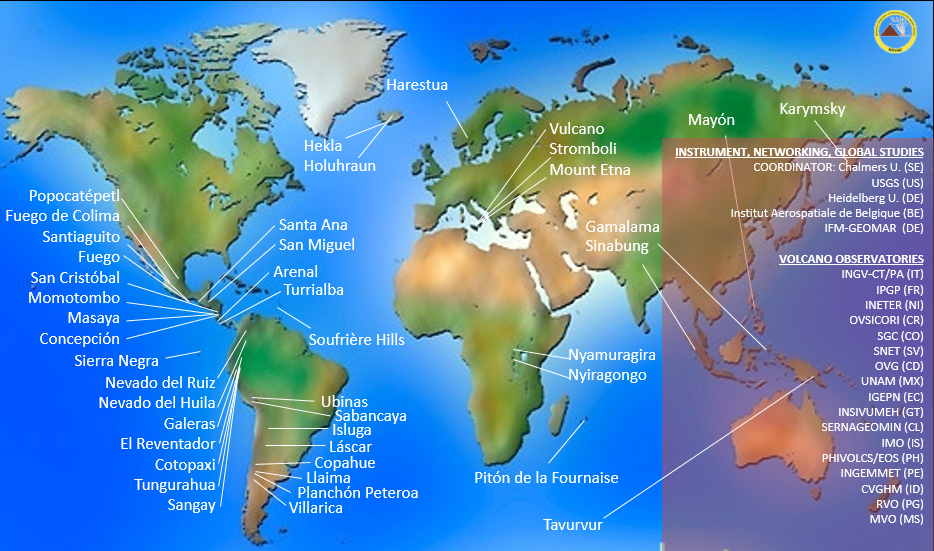
\includegraphics[width=2.1\linewidth]{../../Bilder/NOVACmap}
			\end{column}
			\hspace{2.2cm}
			\begin{column}{.4\textwidth}
				\only<2>{
					\vspace{1.1cm}
					\begin{itemize}
						\item about 40 volcanoes
						\item 2-5 spectrometers at each volcano
					\end{itemize}  }  
				\visible<3>{
						\vspace{1.1cm}
						\begin{itemize}
							\item Primary use of data SO$_2$ flux monitoring
							\item L{\"u}bke et al (2014) also retrieved BrO
							\item BrO close to detection limit
							\item Here we investigate techniques to improve the BrO evaluation from NOVAC data
						\end{itemize}
						}
			\end{column}}
%
		\end{columns}
		
	\end{frame}
	
	
	
	%\begin{frame}
	%\frametitle{\color{mygreen}Network for Observation of Volcanic and Atmospheric Change (NOVAC)\\
	%\color{mygreen}{\rule{0.8\textwidth}{2pt}}}
	%%\setbeamercovered{transparent}
	%
	%  \begin{columns}[T]
	%    \begin{column}{.5\textwidth}
	%
	%% Your image included here
	%    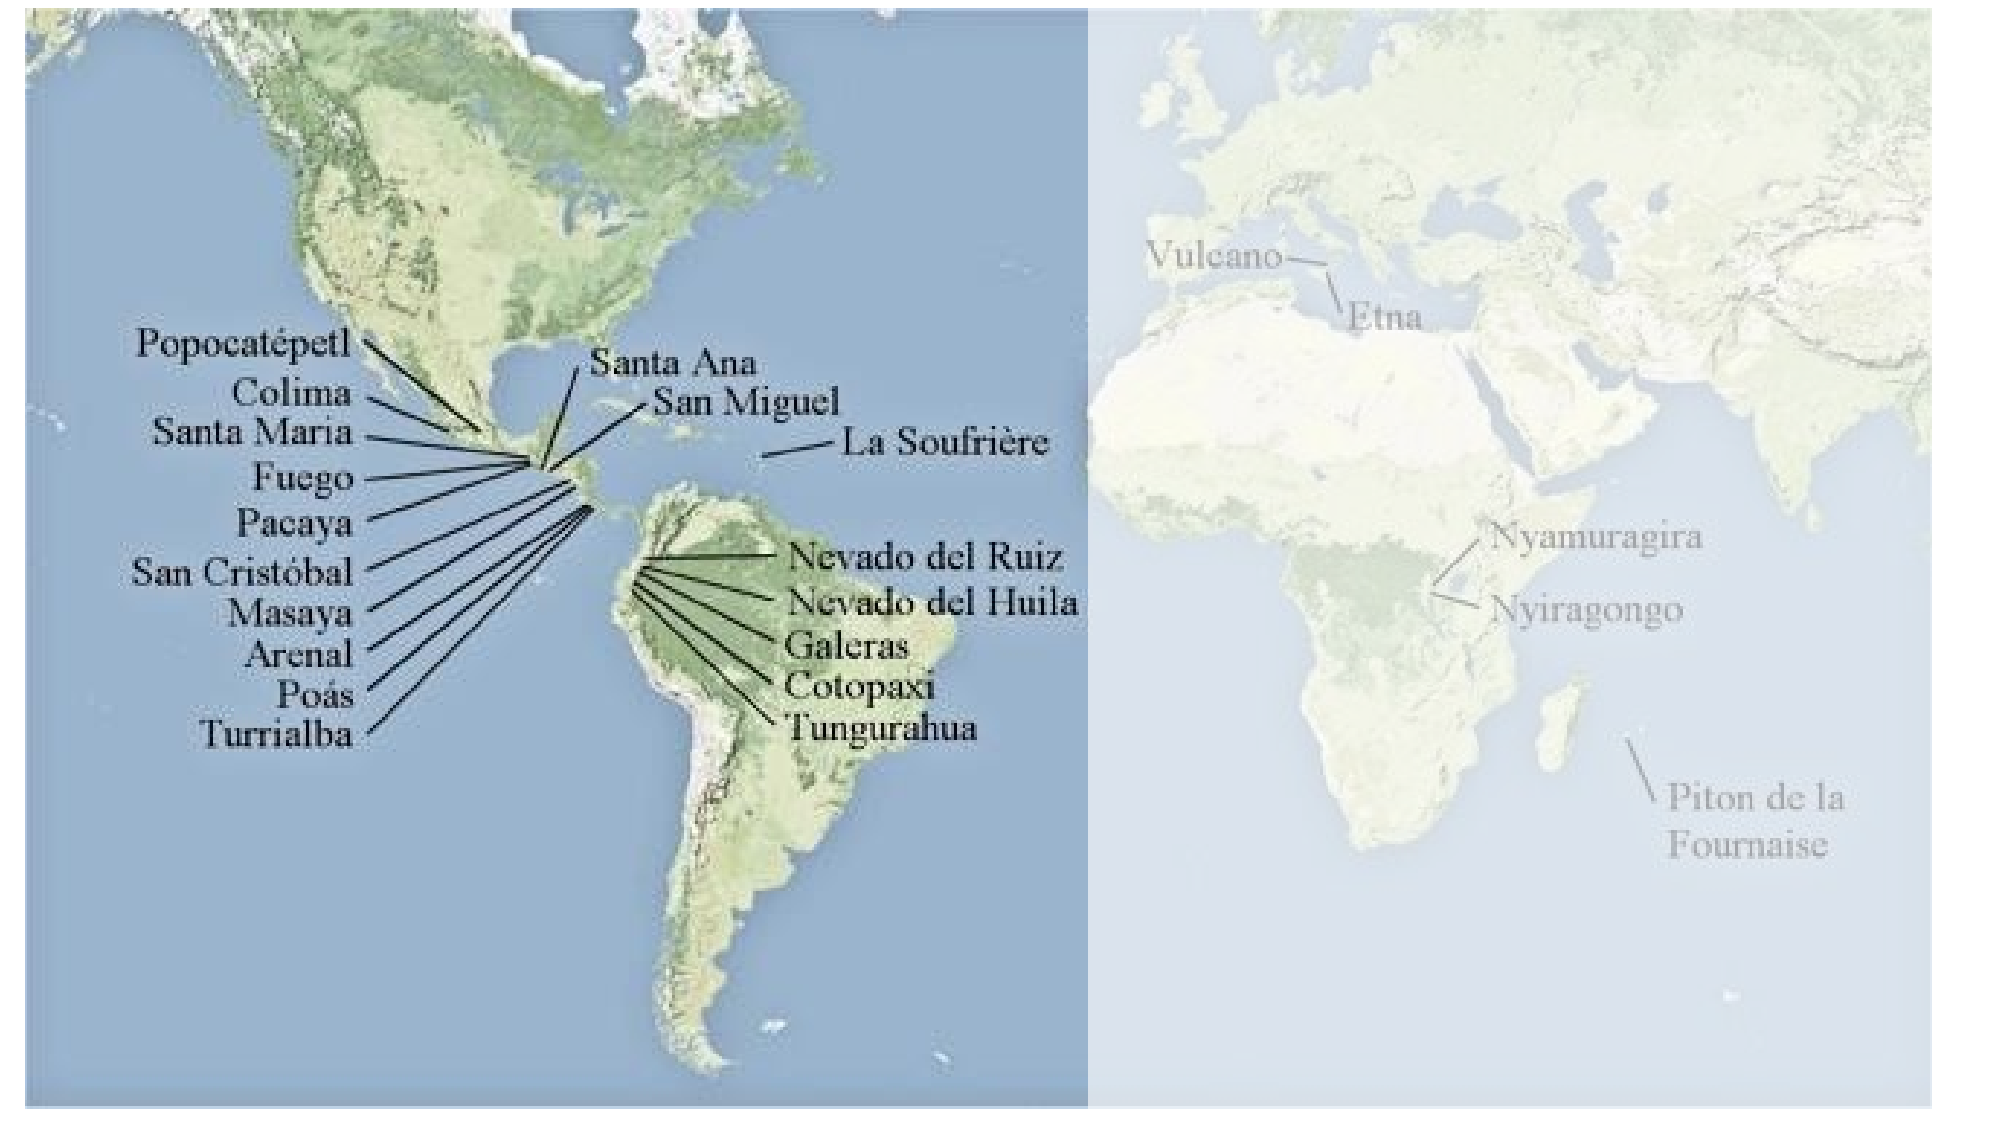
\includegraphics[width=2\linewidth]{../Bilder/Presentation1_3_trans}
	%
	%    \end{column}
	%    
	%
	%    \begin{column}{.5\textwidth}
	%\textbf{
	%	\begin{enumerate}
	%	\item \textit{Initially} founded by European union (2005-2010)
	%	\pause
	%	\item Each volcano is typically monitored with two to four Novac stations.\\
	%	\pause
	%	\item \textit{Location}: typically located 5-10 km downwind
	%	\pause
	%	\item continuous data recording\\
	%	\end{enumerate}
	%}
	%    \end{column}
	%  \end{columns}
	%\end{frame}
	
	
	
	
	
	\begin{frame}
		\frametitle{\color{mygreen}Measurements at Tungurahua\\
			\color{mygreen}{\rule{0.8\textwidth}{2pt}}}
		\vspace{-0.1cm}
		\begin{columns}
			\begin{column}{12cm}
				%\hspace{-2cm}
				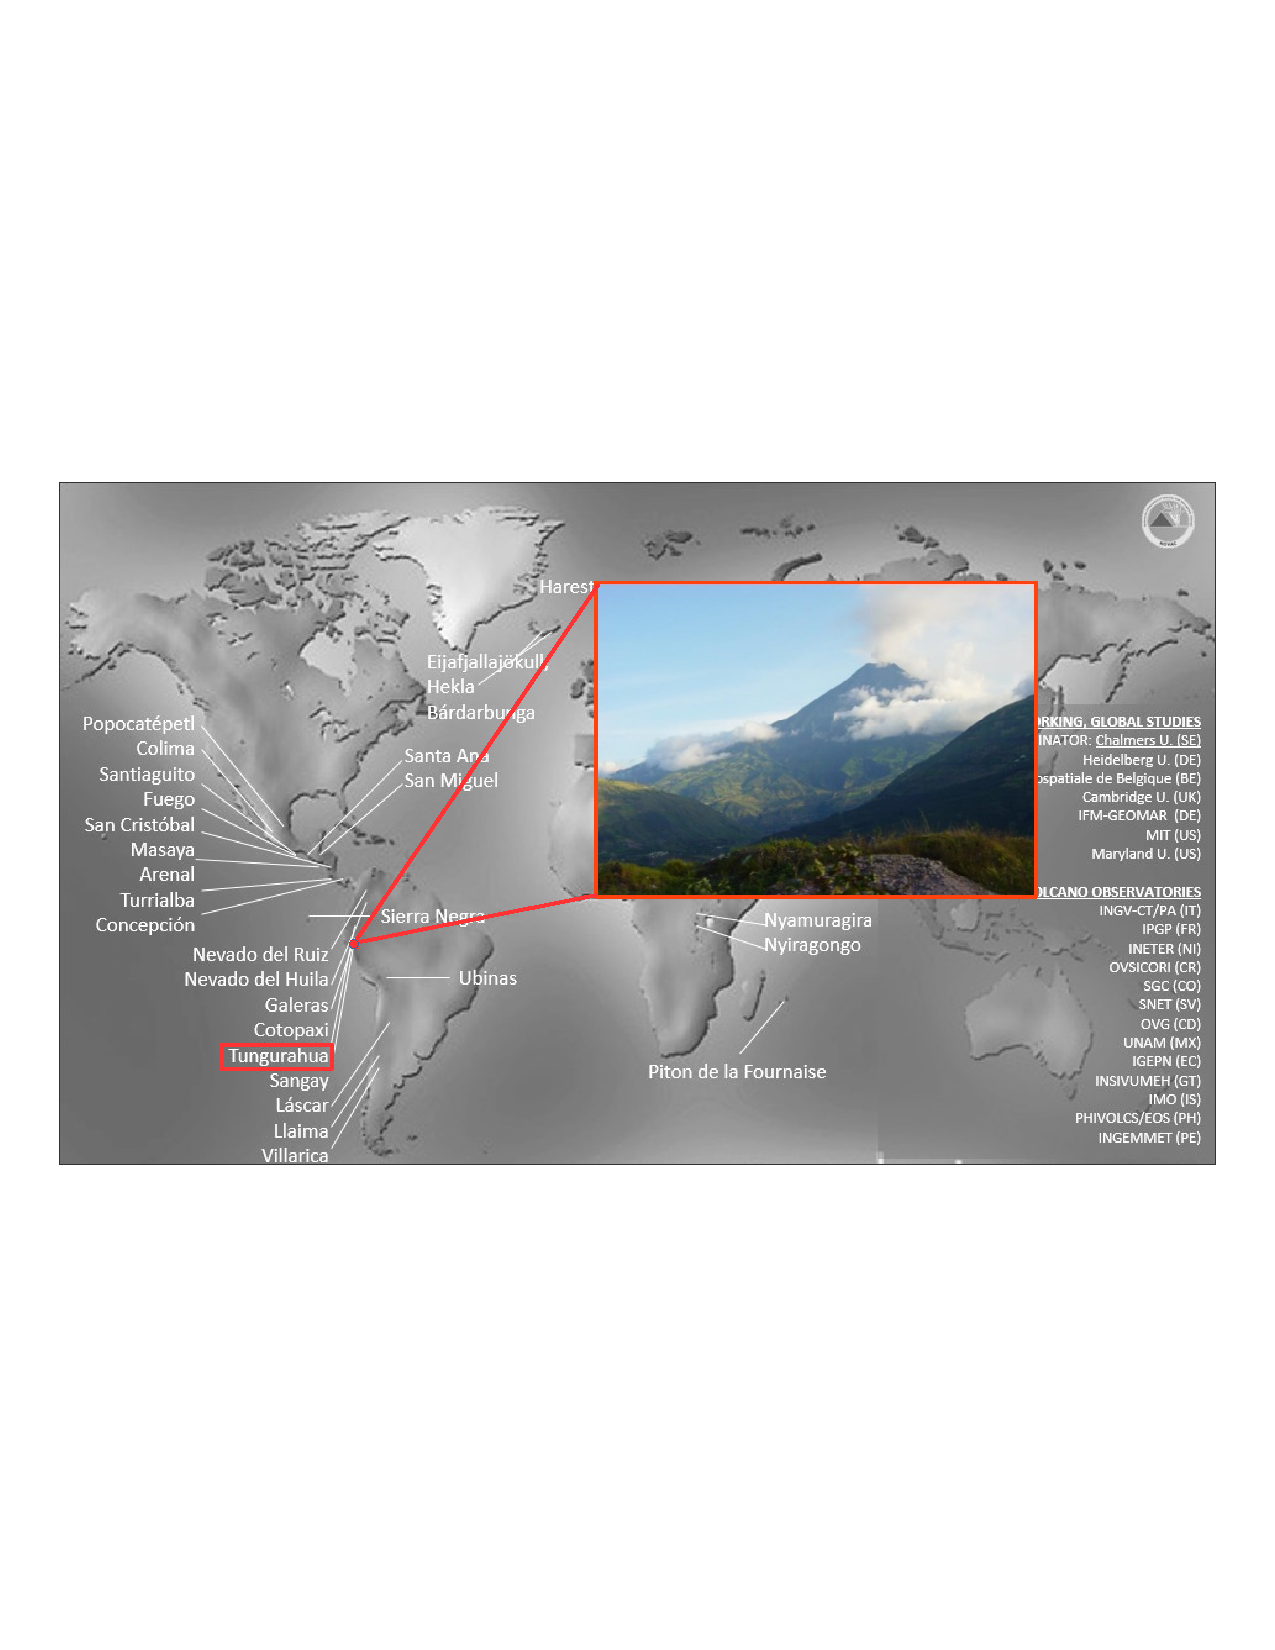
\includegraphics[width=1.0\linewidth]{../../Bilder/NOVAC2015SWTung}
			\end{column}
		\end{columns}
		%
		
	\end{frame}
	
	
	\begin{frame}
		\frametitle{\color{mygreen}One of the NOVAC stations at Tungurahua\\%\rule{_Breite_}{_Stärke_} %%andersrum ist's vertikal;)
			\color{mygreen}{\rule{0.8\textwidth}{2pt}}}
		\vspace{-0.1cm}
		\begin{columns}
			\begin{column}{12cm}
				%\hspace{-2cm}
				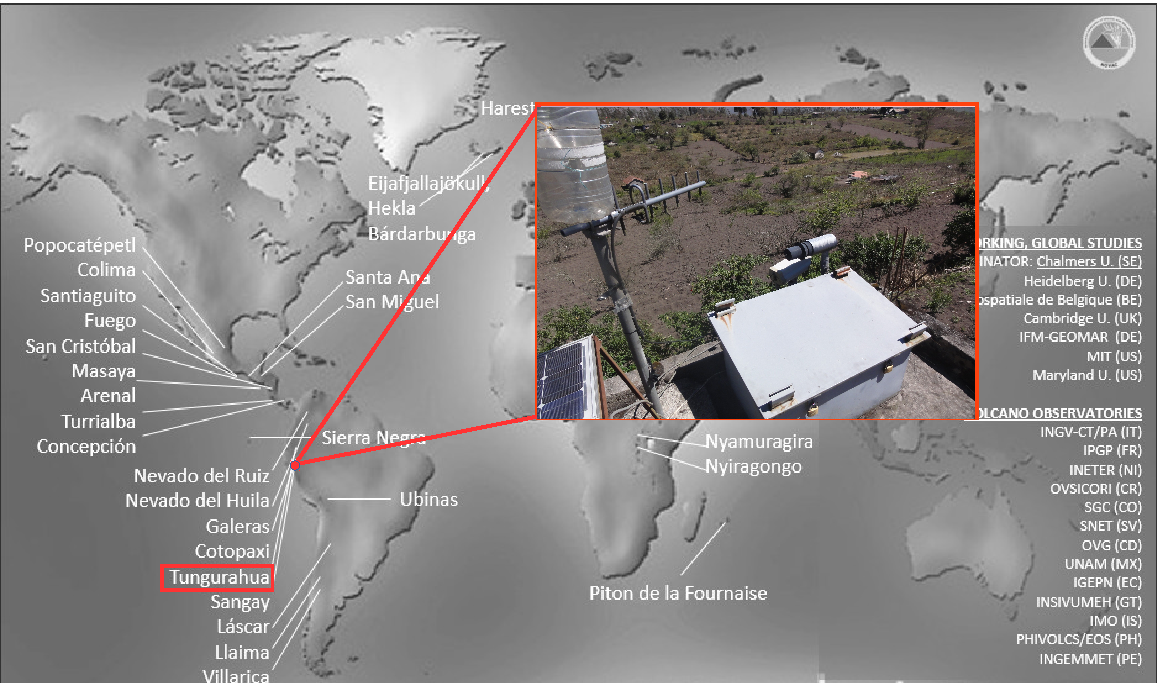
\includegraphics[width=1.\linewidth]{../../Bilder/NOVAC2015SWst}
			\end{column}
		\end{columns}
		
		
	\end{frame}
	
	
	%%----------------------------------------------------------------------------------------
	
	
	\subsection{Differential Optical Absorption Spectroscopy (DOAS)}
	
	
	\begin{frame}
		\frametitle{\color{mygreen}Differential optical absorption spectroscopy (DOAS)\\%\rule{_Breite_}{_Stärke_} %%andersrum ist's vertikal;)
		\color{mygreen}{\rule{0.8\textwidth}{2pt}}}

	\vspace{-1cm}
	\begin{block}{}
		\begin{multicols}{2}
			\textbf{Lambert-Beer Law} \\
			\vspace{-0.5cm}
			\begin{equation*}
			\hspace*{-0.9cm}I\left(\lambda \right) = I^{'}_{0}\left(\lambda\right)\cdot exp\left(\sum_{i}\sigma_{i}\cdot c_{i}\cdot L \right)
			\end{equation*}
			\textbf{Optical density}
			\vspace{-0.5cm}
			\begin{equation*}
			\tau_{i} = ln\left(\frac{I(\lambda)}{I^{'}_{0}\left(\lambda\right)}\right) = S\cdot\sigma_{i}
			\end{equation*}
		\end{multicols}	
	\end{block}
	\begin{multicols}{2}
		\begin{figure}
			\centering
			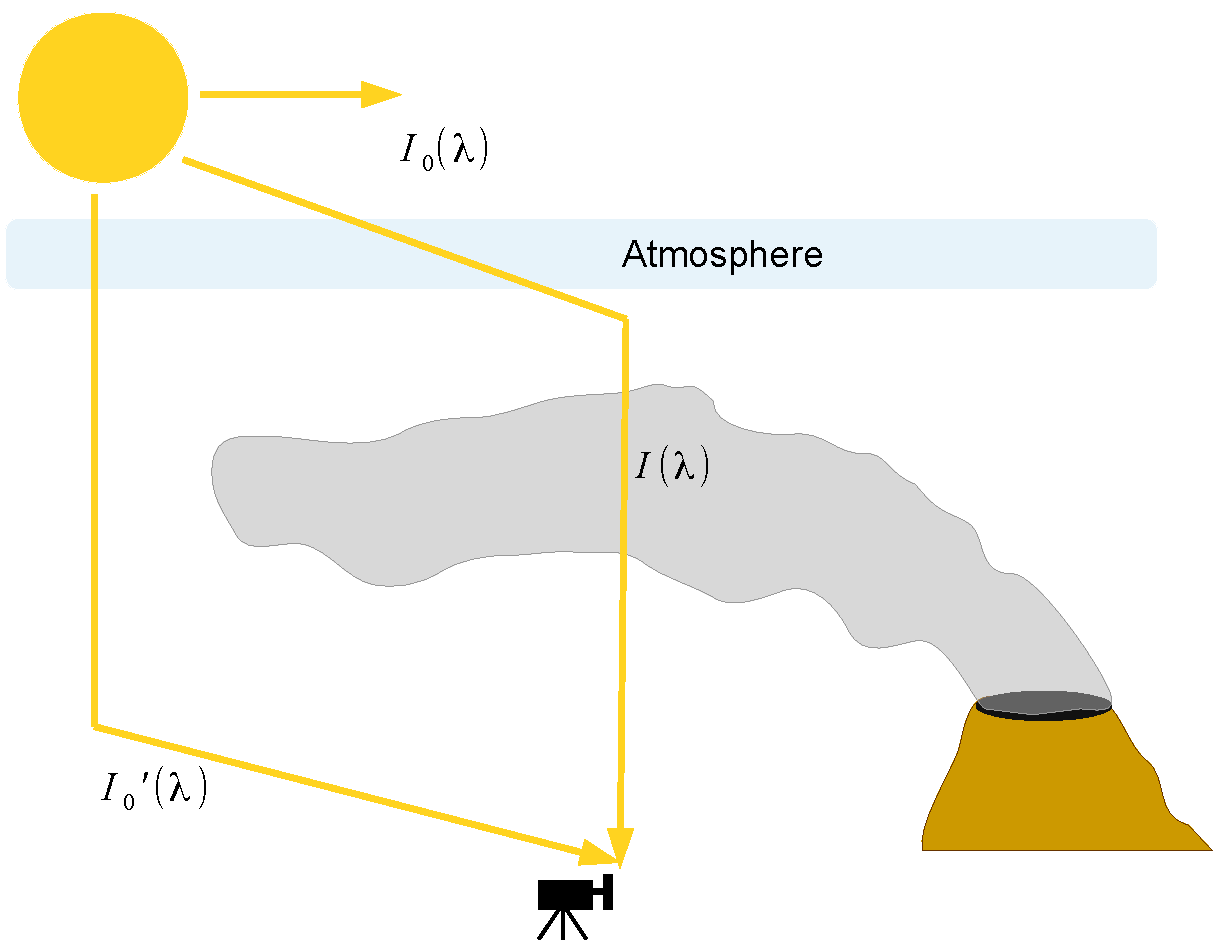
\includegraphics[width=1\linewidth]{../../Bilder/DOASFunction}
			\label{fig:doasfunction}
		\end{figure}
	\begin{figure}
		\centering
		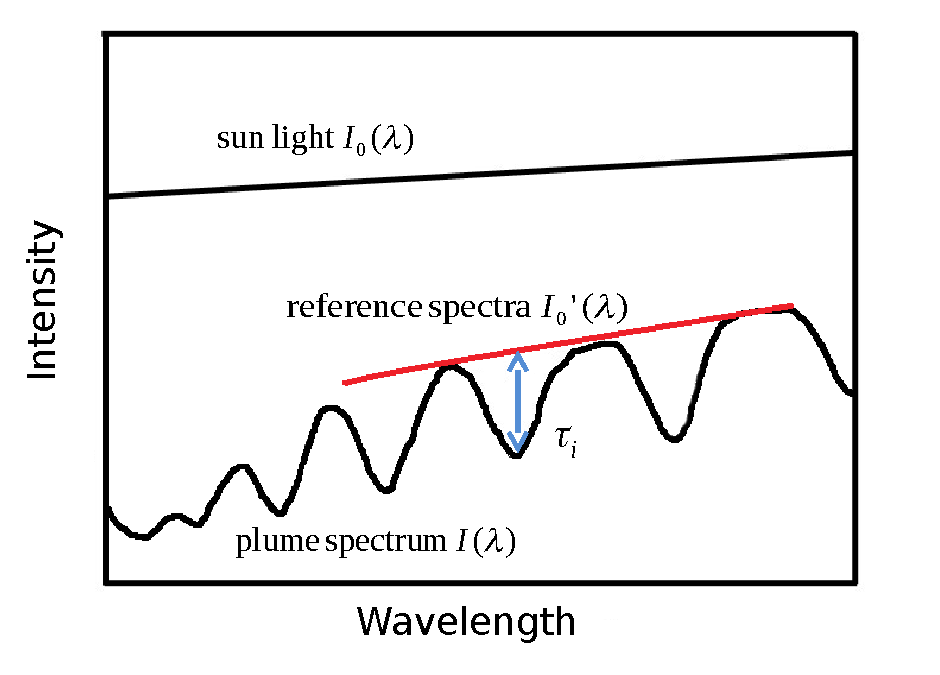
\includegraphics[width=1\linewidth]{../../Bilder/dddd}
		\label{fig:dddd}
	\end{figure}	
	\end{multicols}
	\end{frame}



	\begin{frame}
\frametitle{\color{mygreen}Multi Axis DOAS at NOVAC\\%\rule{_Breite_}{_Stärke_} %%andersrum ist's vertikal;)
	\color{mygreen}{\rule{0.8\textwidth}{2pt}}}

\vspace{-1cm}
\begin{block}{}
	\begin{multicols}{2}
		\textbf{Lambert-Beer Law} \\
		\vspace{-0.5cm}
		\begin{equation*}
		\hspace*{-0.9cm}I\left(\lambda \right) = I^{'}_{0}\left(\lambda\right)\cdot exp\left(\sum_{i}\sigma_{i}\cdot c_{i}\cdot L \right)
		\end{equation*}
		\textbf{Optical density}
		\vspace{-0.5cm}
		\begin{equation*}
		\tau_{i} = ln\left(\frac{I(\lambda)}{I^{'}_{0}\left(\lambda\right)}\right) = S\cdot\sigma_{i}
		\end{equation*}
	\end{multicols}	
\end{block}
\begin{multicols}{2}
	\begin{figure}
		\centering
		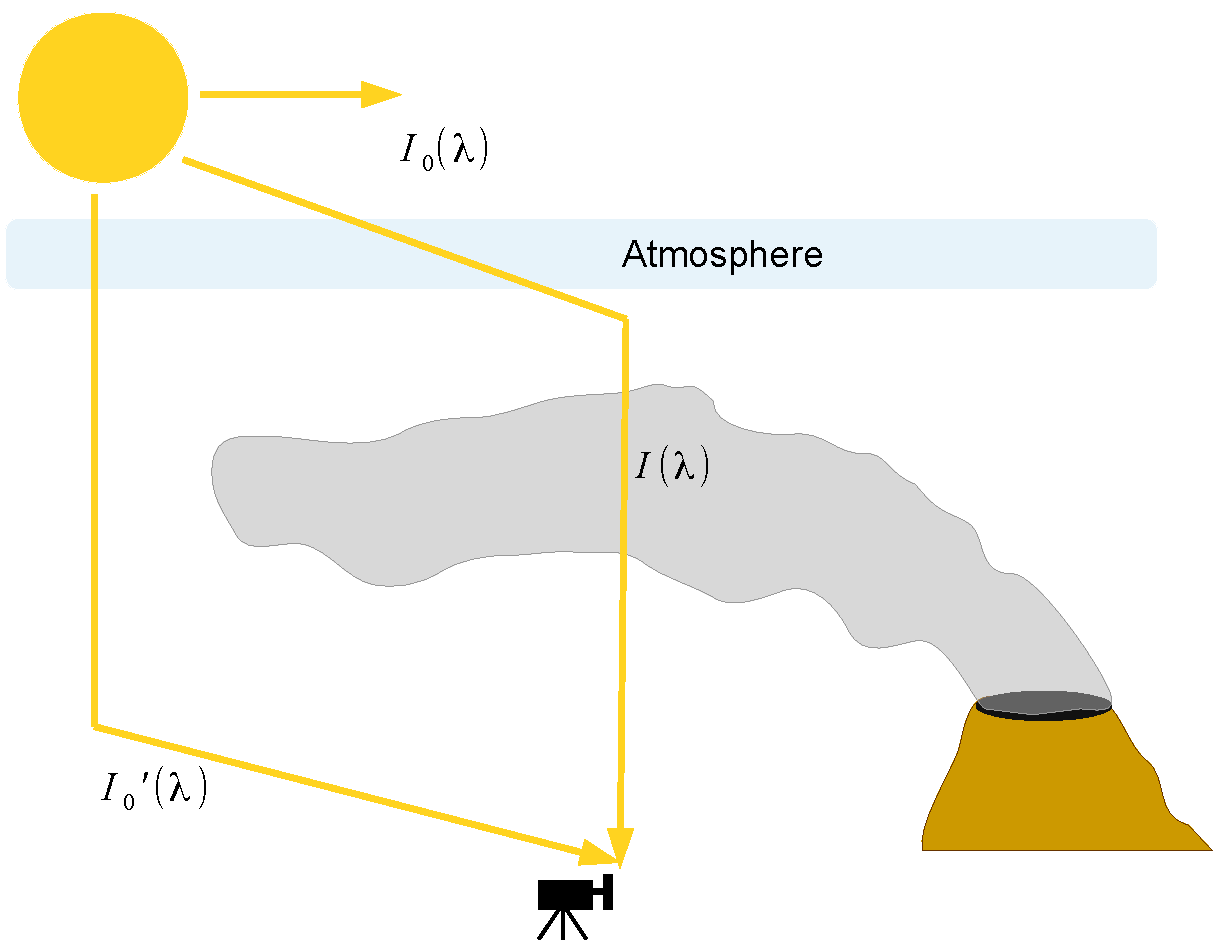
\includegraphics[width=1\linewidth]{../../Bilder/DOASFunction}
		\label{fig:doasfunction}
	\end{figure}
	\begin{figure}
		\centering
		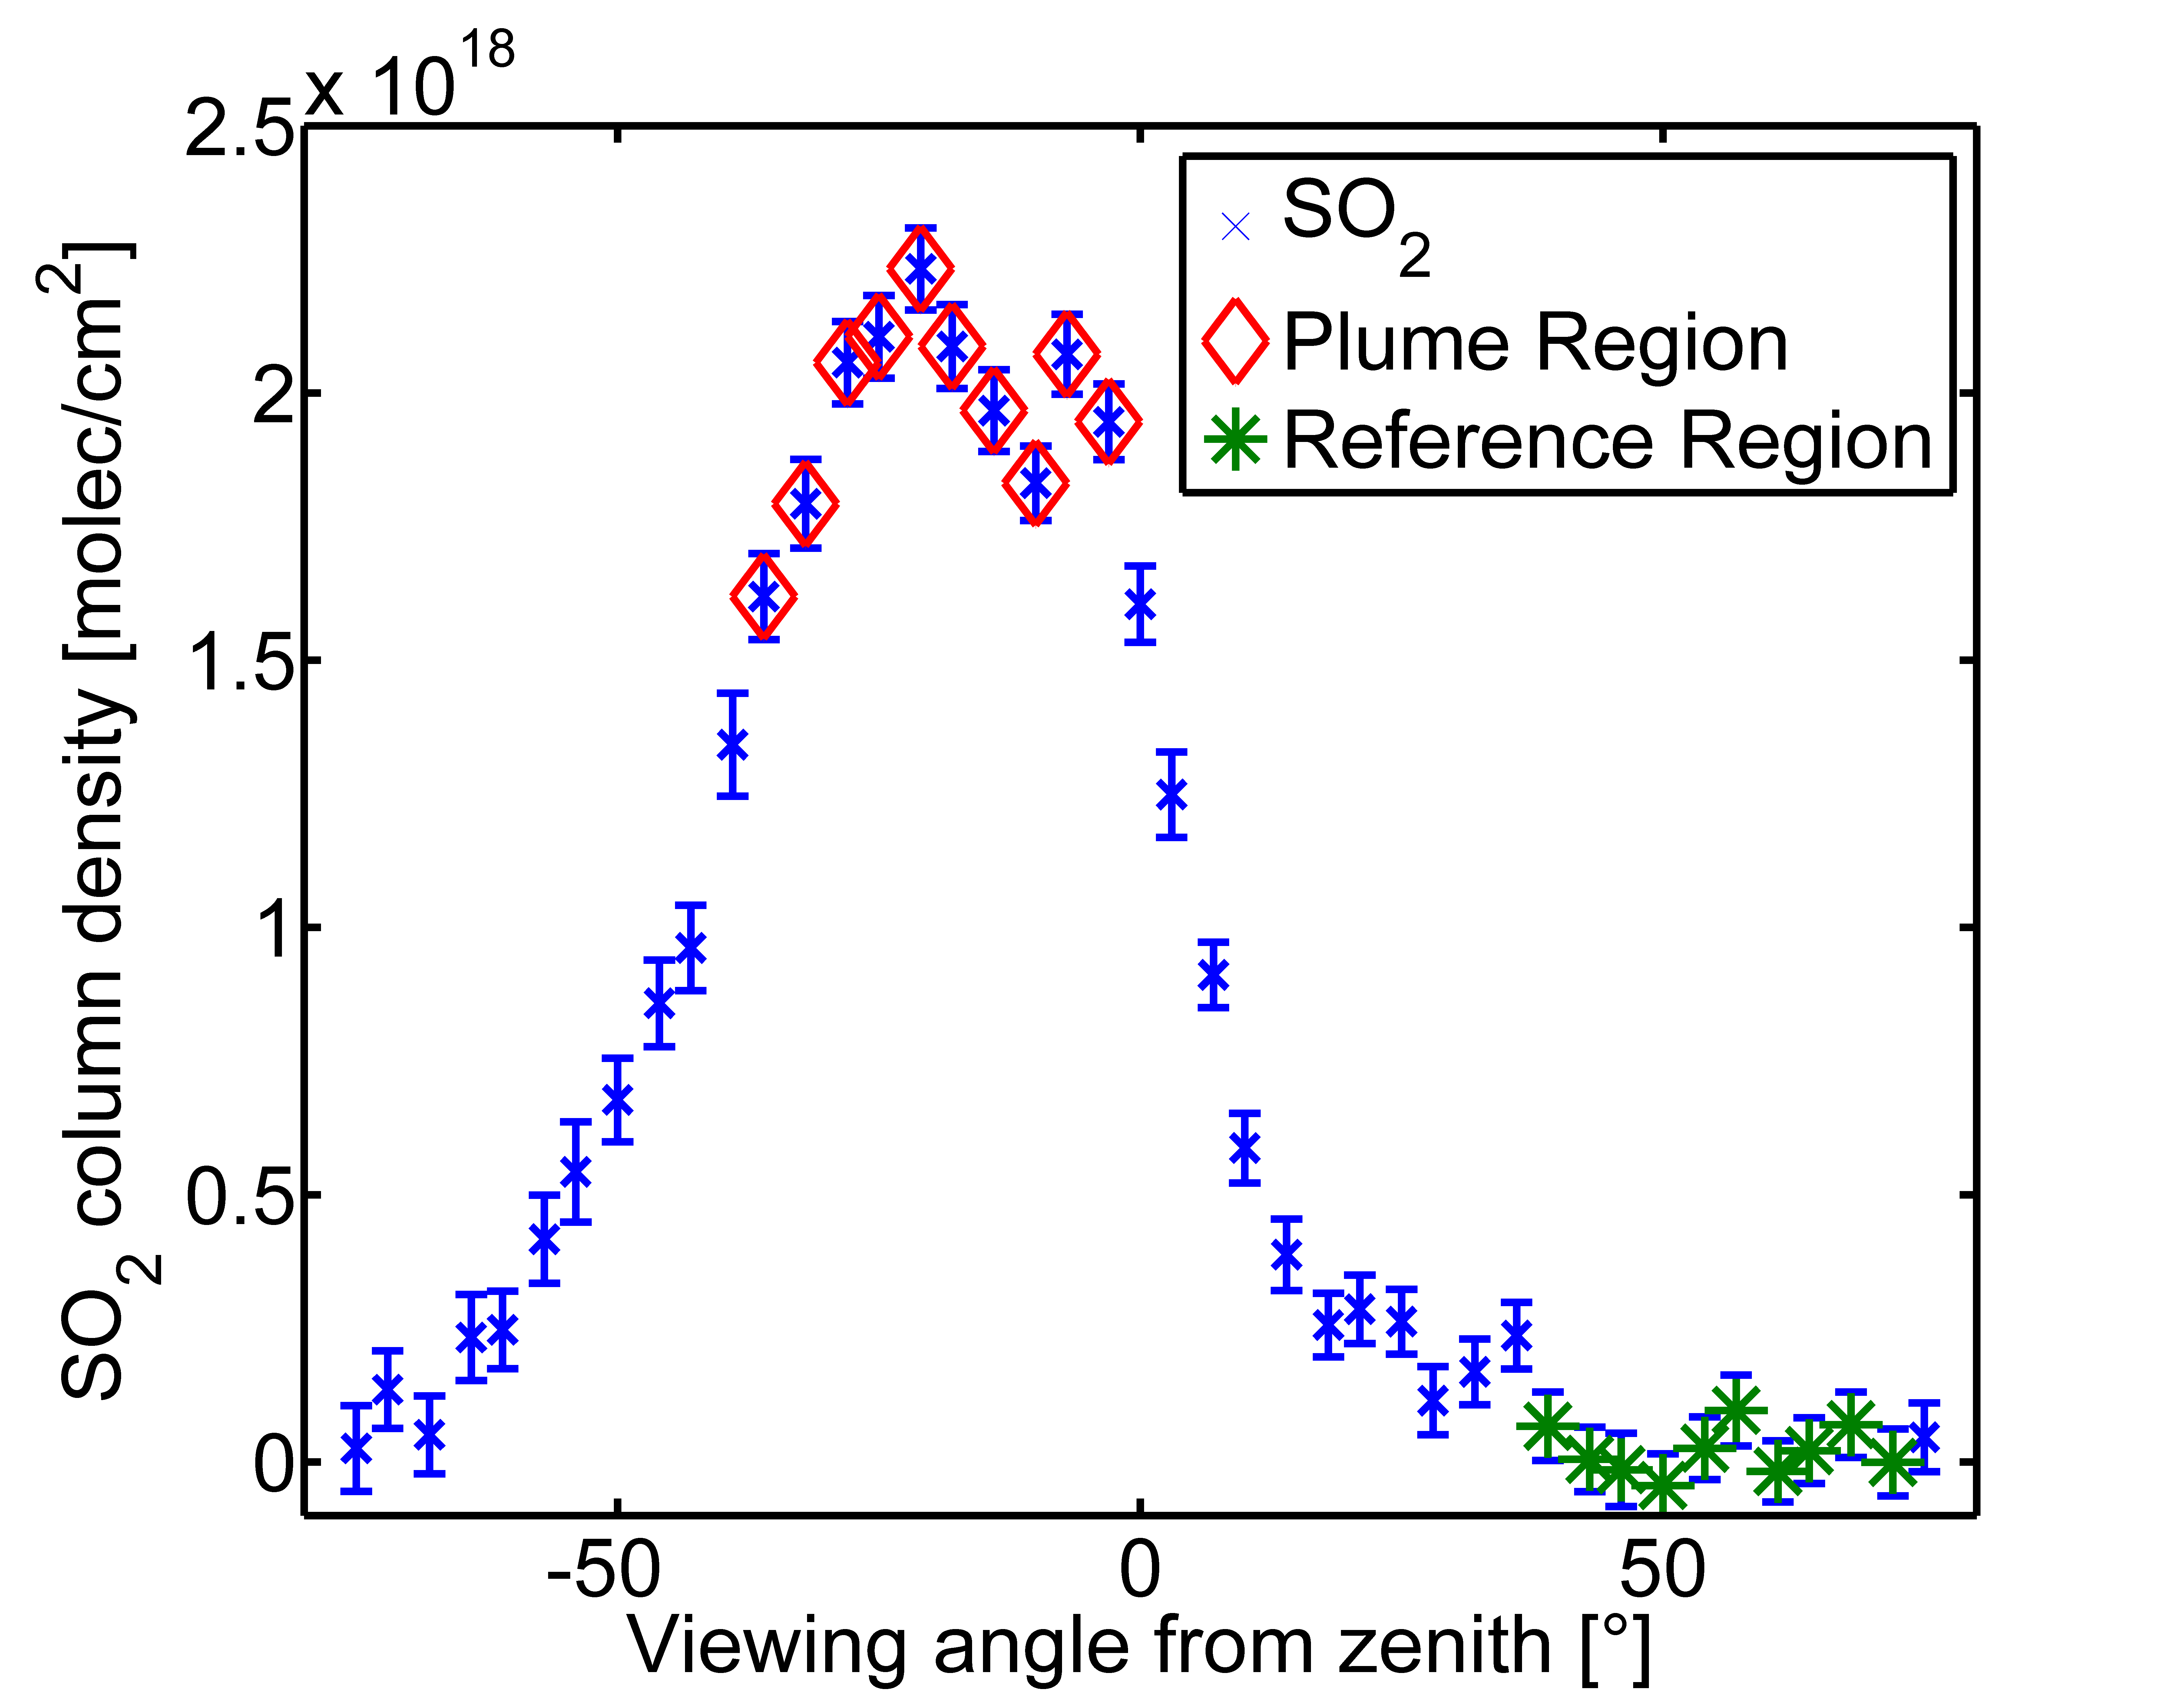
\includegraphics[width=1\linewidth]{../../Bilder/SO2_Scan}
		\label{fig:dddd}
	\end{figure}	
\end{multicols}
\end{frame}





	
	\begin{frame}
		\frametitle{\color{mygreen}Contamination\\%\rule{_Breite_}{_Stärke_} %%andersrum ist's vertikal;)
		\color{mygreen}{\rule{0.8\textwidth}{2pt}}}
		\begin{figure}
			\centering
			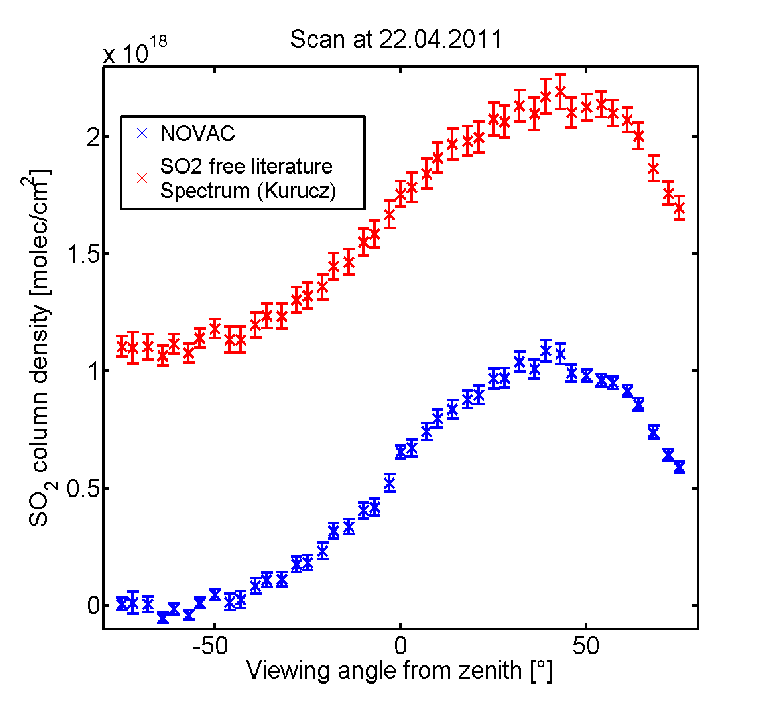
\includegraphics[width=0.7\linewidth]{../../Bilder/contaminated}
			\caption{}
			\label{fig:contaminated}
		\end{figure}
	
	\end{frame}	
	

			

		\begin{frame}
			\frametitle{\color{mygreen} Checking for contamination\\%\rule{_Breite_}{_Stärke_} %%andersrum ist's vertikal;)
				\color{mygreen}{\rule{0.8\textwidth}{2pt}}}
			\vspace{-0.2cm}
			\begin{itemize}
				\item Possible contaminations can be checked
				by a theoretical solar atlas spectrum to evaluate the \ce{SO2} amount in the reference.
				\item Data are contaminated if the \ce{SO2} amount in the reference is above $2\cdot 10^{17}$ 
				\item Only accept \ce{SO2} SCDs above the plume limit of $7\cdot 10^{17} \frac{molec}{cm^2}$
			\end{itemize}
		\end{frame}
		%%--------------------------------------------------------
		
		\section{Influences on Reference}
		\begin{frame}
			\frametitle{\color{mygreen}Temporal difference between the reference and the plume \\%\rule{_Breite_}{_Stärke_} %%andersrum ist's vertikal;)
				\color{mygreen}{\rule{0.8\textwidth}{2pt}}}
			\vspace{-0.2cm}
			\begin{multicols}{2}
				
				\begin{figure}
					\centering
					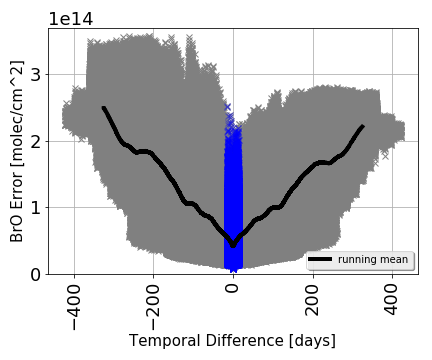
\includegraphics[width=1.05\linewidth]{../../Bilder/Datum}
					\label{fig:Datum}
				\end{figure}
				\newpage
				\vspace*{0.5cm}
				\begin{itemize}
					\item Increase of BrO error with temporal difference
					\item The sign of the temporal difference irrelevant
					\item Restrict temporal difference to two weeks
				\end{itemize}
			\end{multicols}
			
		\end{frame}
		
		\begin{frame}
			\frametitle{\color{mygreen}Influence of ambient conditions on BrO measurement error\\%\rule{_Breite_}{_Stärke_} %%andersrum ist's vertikal;)
				\color{mygreen}{\rule{0.8\textwidth}{2pt}}}
			\vspace{-0.2cm}
			\begin{multicols}{2}
				
				\begin{figure}[htbp] 
					%\begin{minipage}[t]{0.5\textwidth}
					
					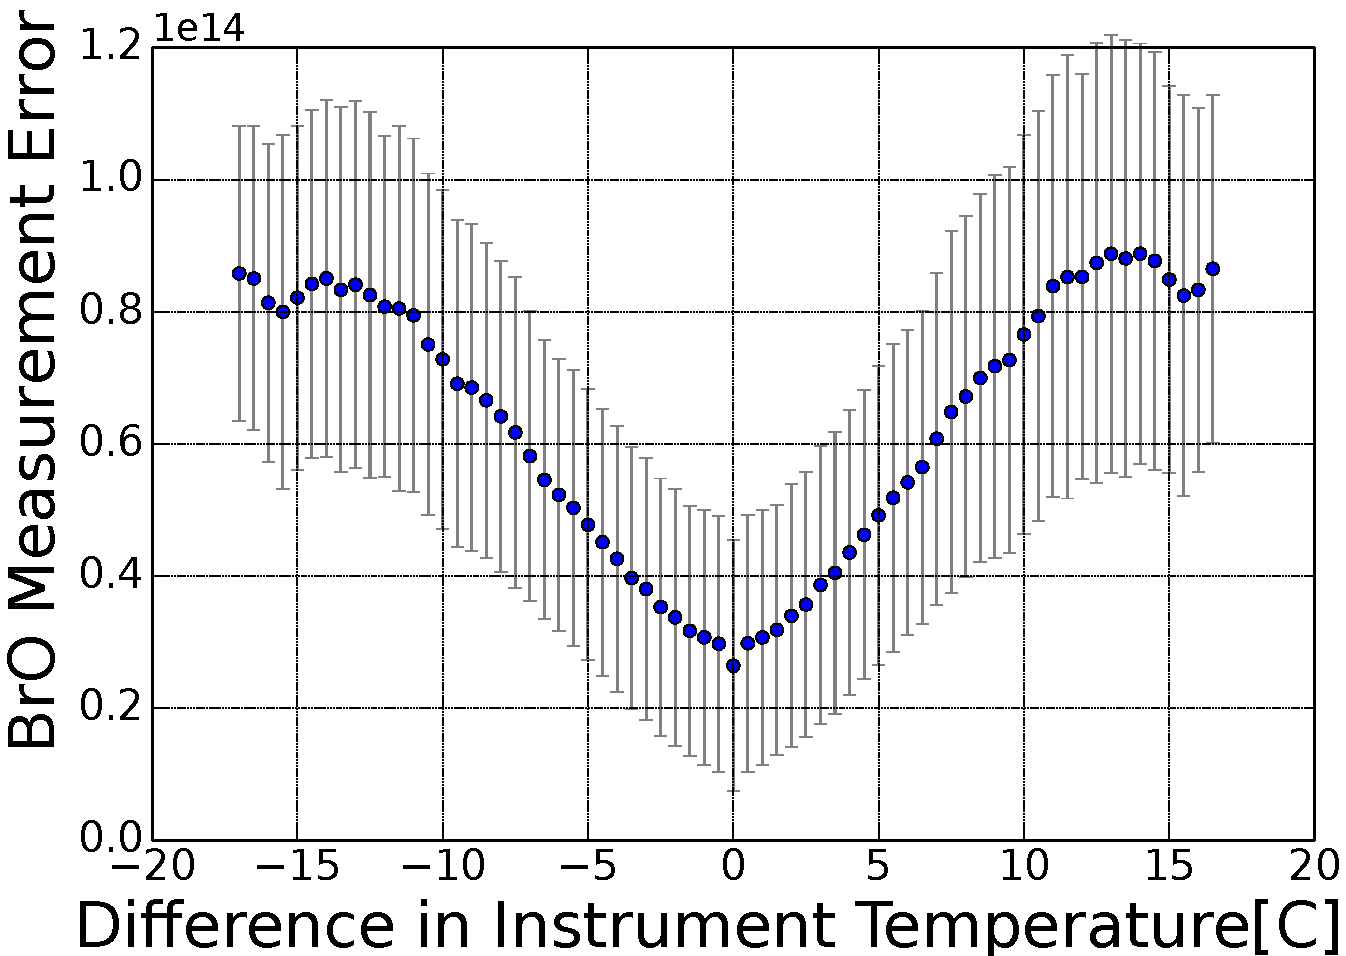
\includegraphics[width=5cm]{../../Bilder/Differcence_inTemperature[C]}
					%\end{minipage}
					\vspace{0.01cm}
					%\begin{minipage}[t]{0.5\textwidth}
					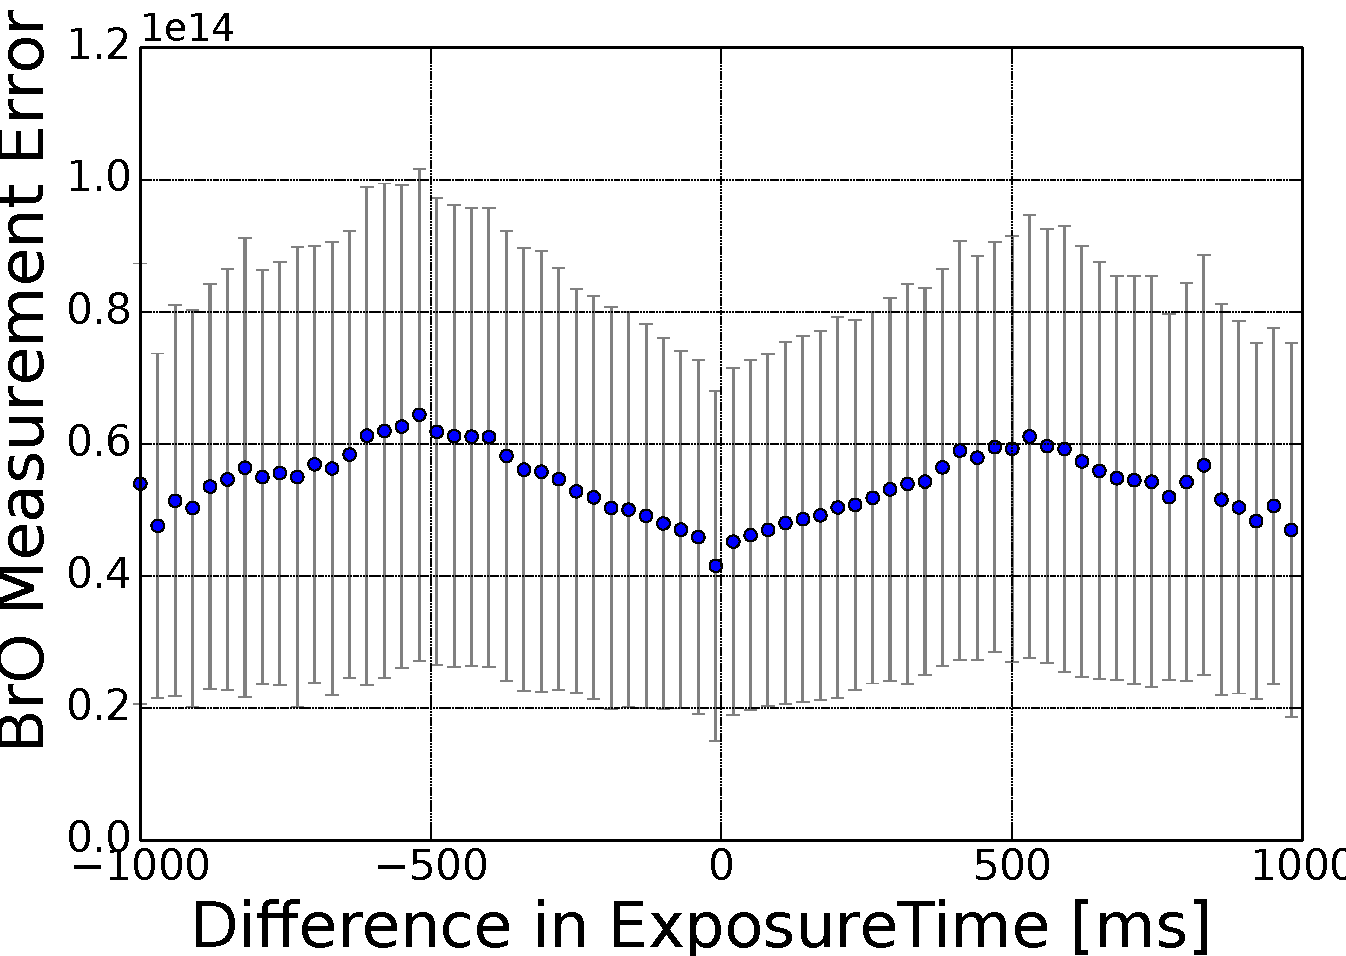
\includegraphics[width=5cm]{../../Bilder/Differcence_inExposureTime[ms]}
					%\end{minipage}
				\end{figure}
				\begin{figure}[htbp] 
					%\begin{minipage}[t]{0.5\textwidth}
					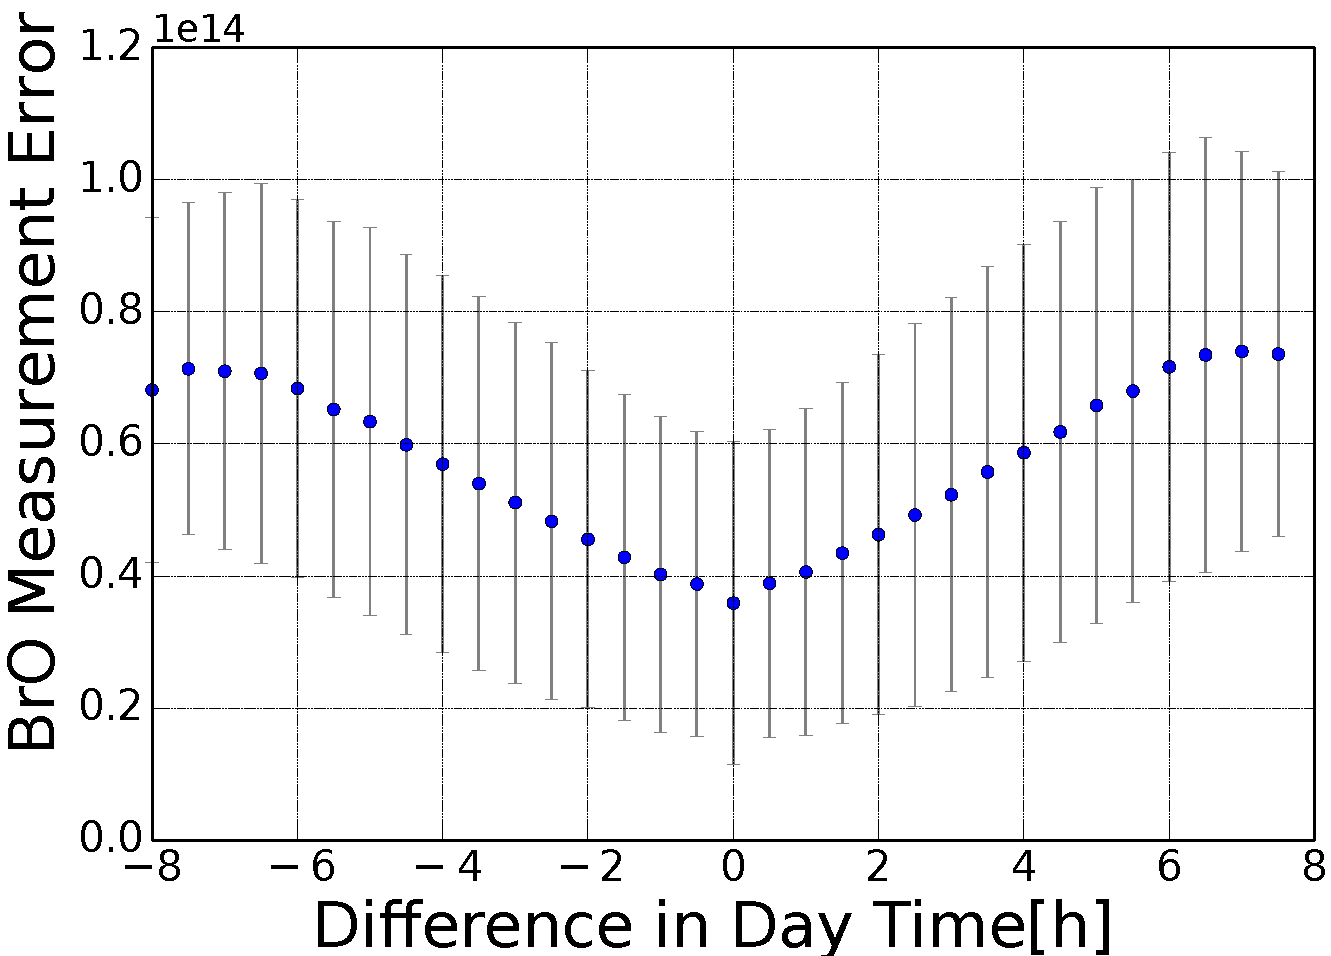
\includegraphics[width=5cm]{../../Bilder/Differcence_in_DayTime[h]a}
					%\end{minipage}
					\vspace{0.01cm}
					%\begin{minipage}[t]{0.5\textwidth}
					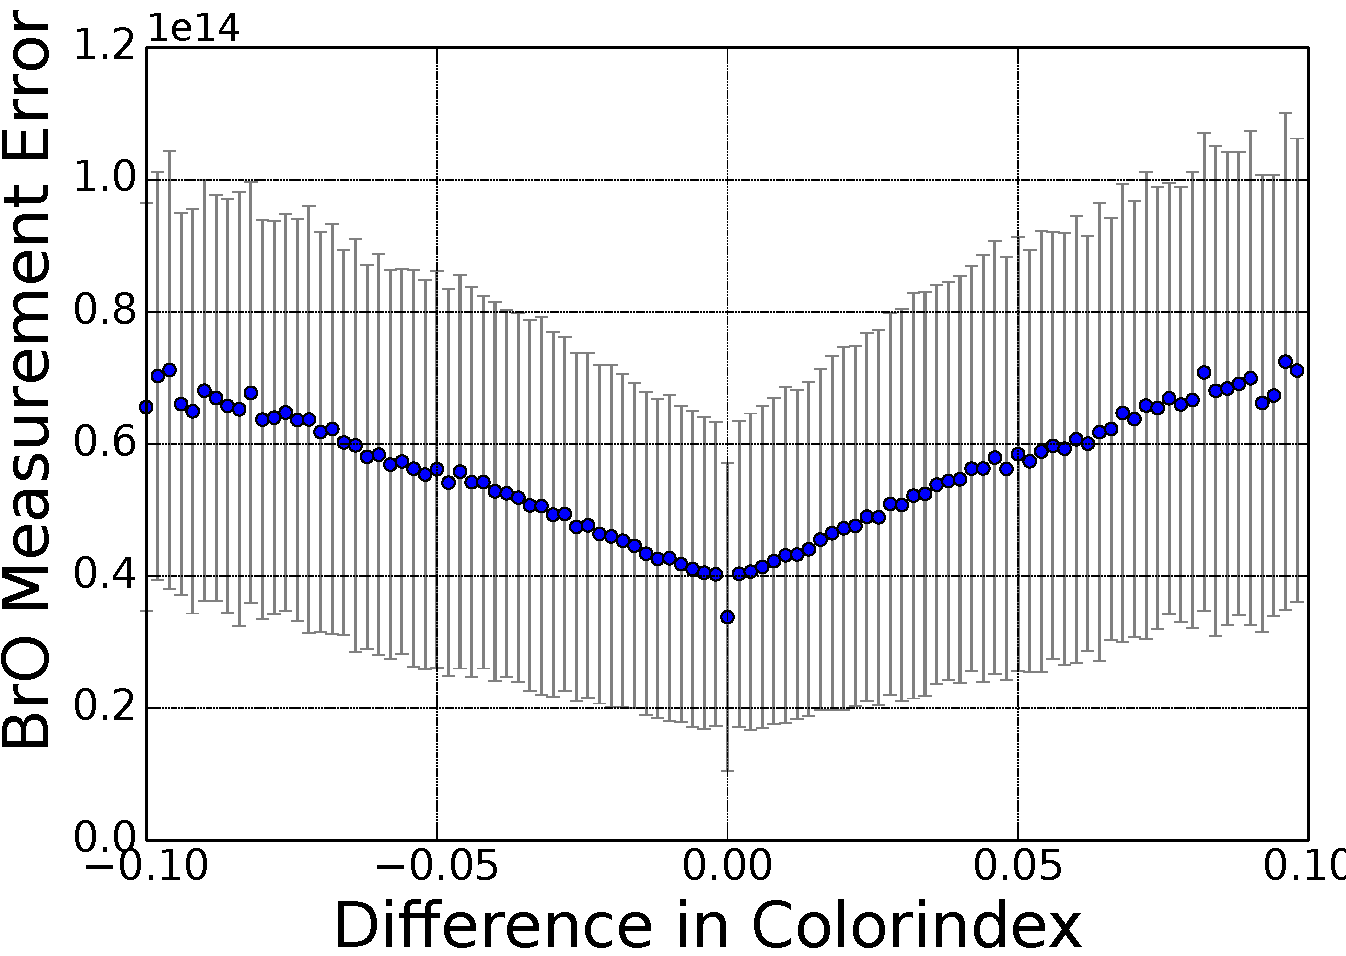
\includegraphics[width=5cm]{../../Bilder/Differcence_inColorindex}
					%\end{minipage}
				\end{figure}
				
			\end{multicols}
		\end{frame}
		
		%------------------------------------------------
		
		
		\section{All year Data}
		\begin{frame}
			\frametitle{\color{mygreen}Comparison of the different evaluations - SO$_2$\\%\rule{_Breite_}{_Stärke_} %%andersrum ist's vertikal;)
				\color{mygreen}{\rule{0.8\textwidth}{2pt}}}
			\begin{figure}[h!]	
				\subfigure[Data of Tungurahua]{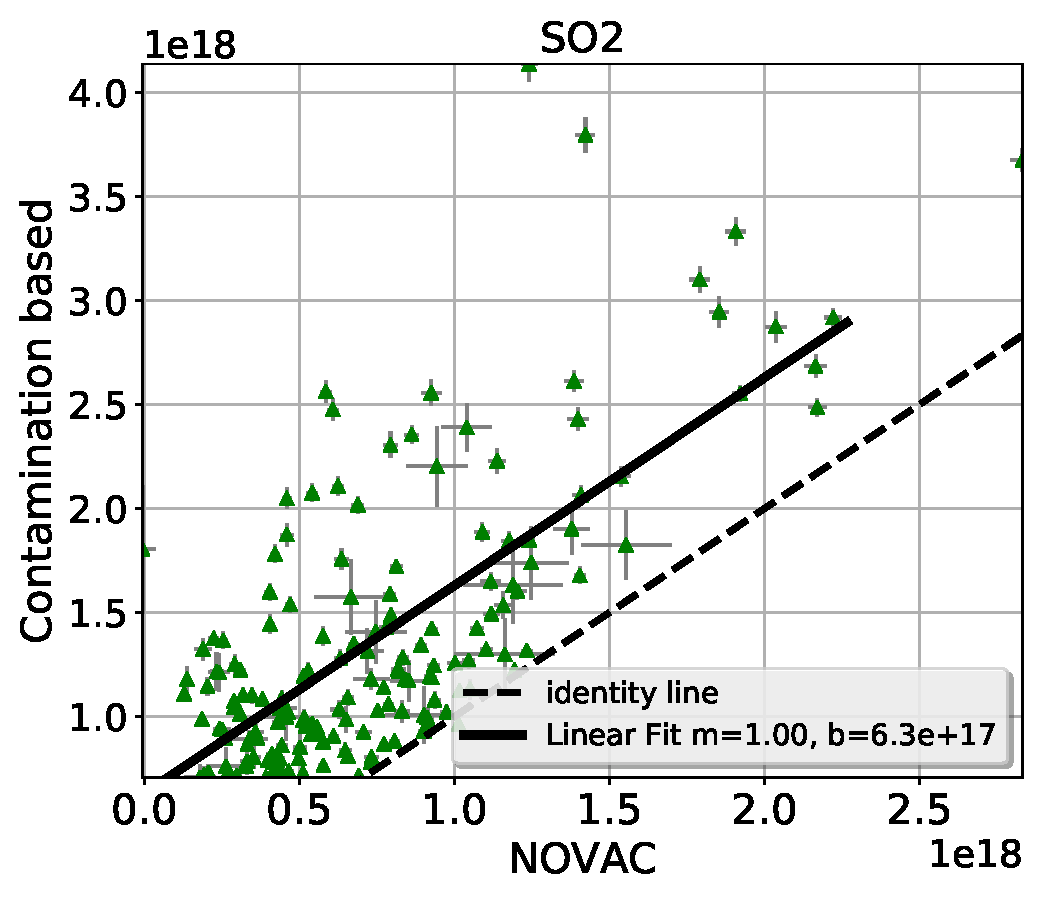
\includegraphics[width=0.49\textwidth]{../../Bilder/tung_so2_novac_conbased}}
				\subfigure[Data of Nevado Del Riz]{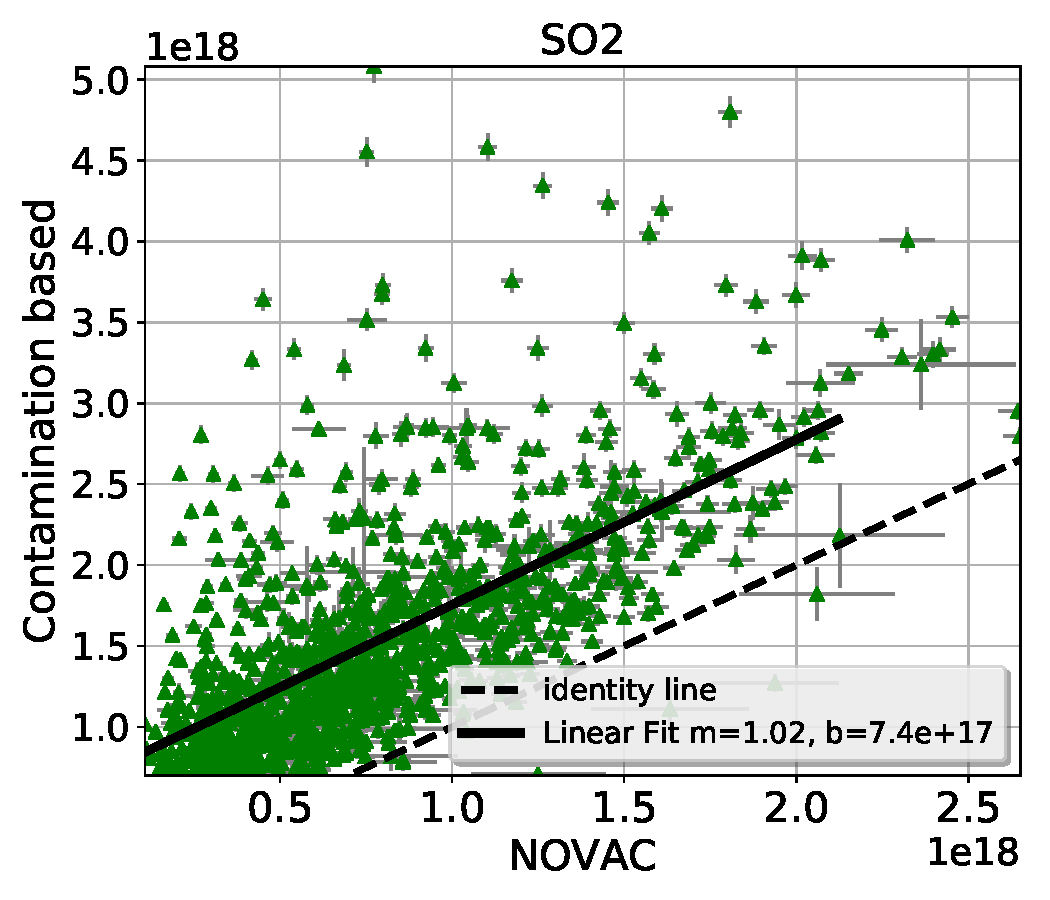
\includegraphics[width=0.49\textwidth]{../../Bilder/so2_novac_conbased}}
			\end{figure}
			\pause
			\begin{multicols}{2}
				\begin{itemize}
					\item Contamination lead to a offset on \ce{SO2} SCDs\\
					\newpage
					\pause
					\item Behavior at Tungurahua and Nevado Del Ruiz is equivalent
				\end{itemize}
			\end{multicols}
		\end{frame}
		
		\begin{frame}
			\frametitle{\color{mygreen}Comparison of the different evaluations - BrO\\%\rule{_Breite_}{_Stärke_} %%andersrum ist's vertikal;)
				\color{mygreen}{\rule{0.8\textwidth}{2pt}}}
			\begin{figure}[h!]	
				\subfigure[Data of Tungurahua]{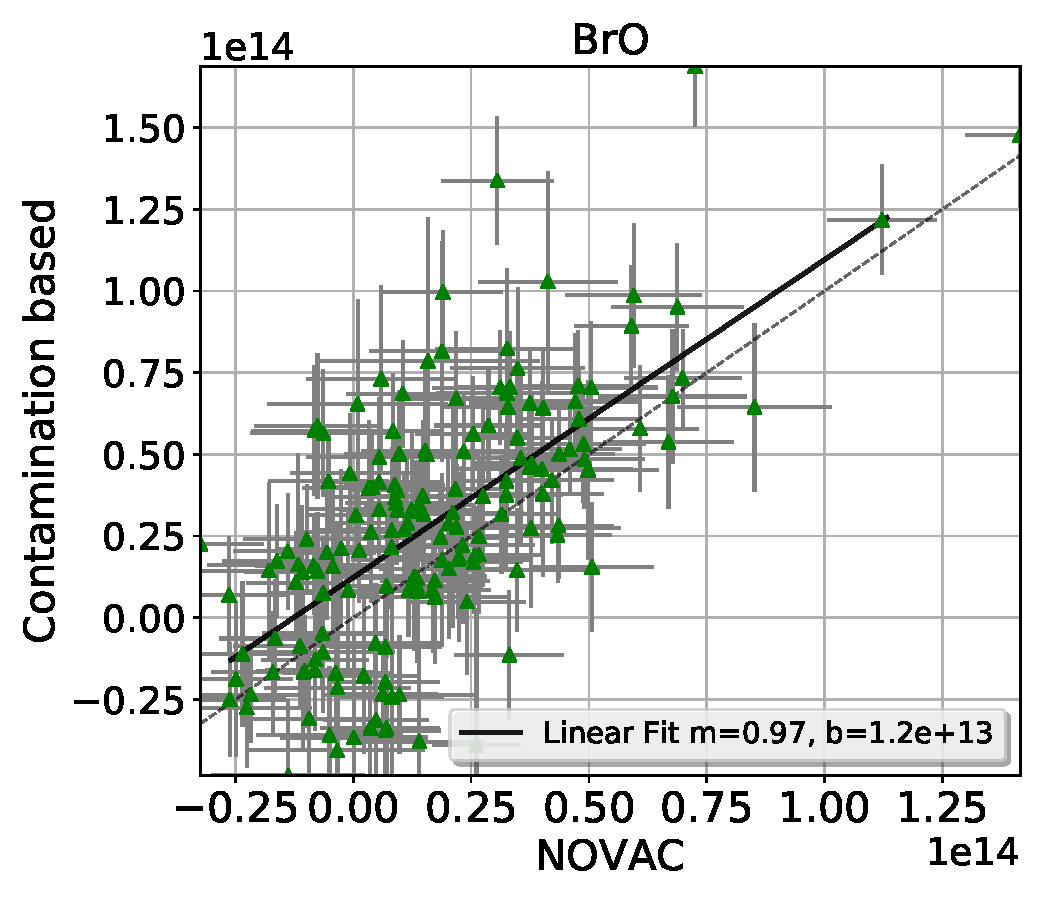
\includegraphics[width=0.49\textwidth]{../../Bilder/tung_bro_novac_conbased}}
				\subfigure[Data of Nevado Del Riz]{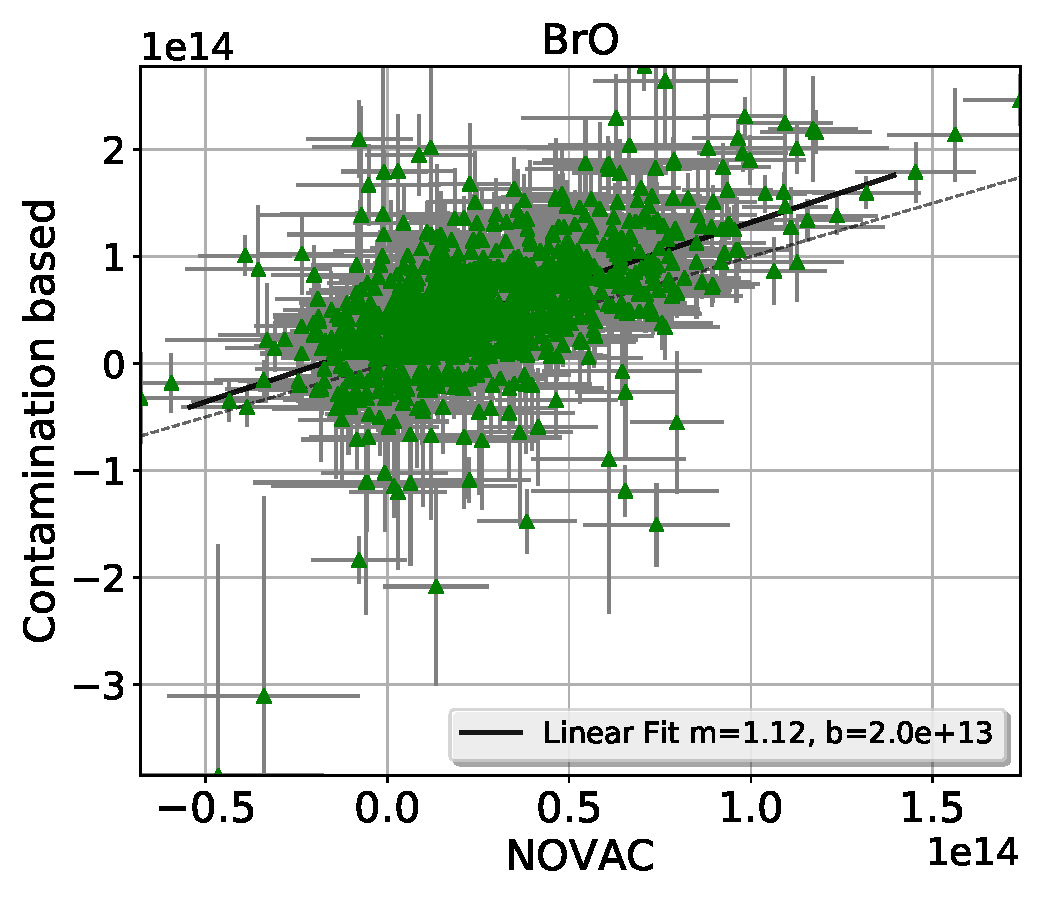
\includegraphics[width=0.49\textwidth]{../../Bilder/bro_novac_conbased}}
			\end{figure}
			\pause
			\begin{multicols}{2}
				\begin{itemize}
					\item  Contamination lead to a offset on BrO SCDs\\ 
					\pause
					\item proportional BrO increase lower as for \ce{SO2}
				\end{itemize}
			\end{multicols}
		\end{frame}
		
		\begin{frame}
			\frametitle{\color{mygreen}Comparison of the different evaluations - BrO/SO$_2$\\%\rule{_Breite_}{_Stärke_} %%andersrum ist's vertikal;)
				\color{mygreen}{\rule{0.8\textwidth}{2pt}}}
			\begin{figure}[h!]	
				\subfigure[Data of Tungurahua]{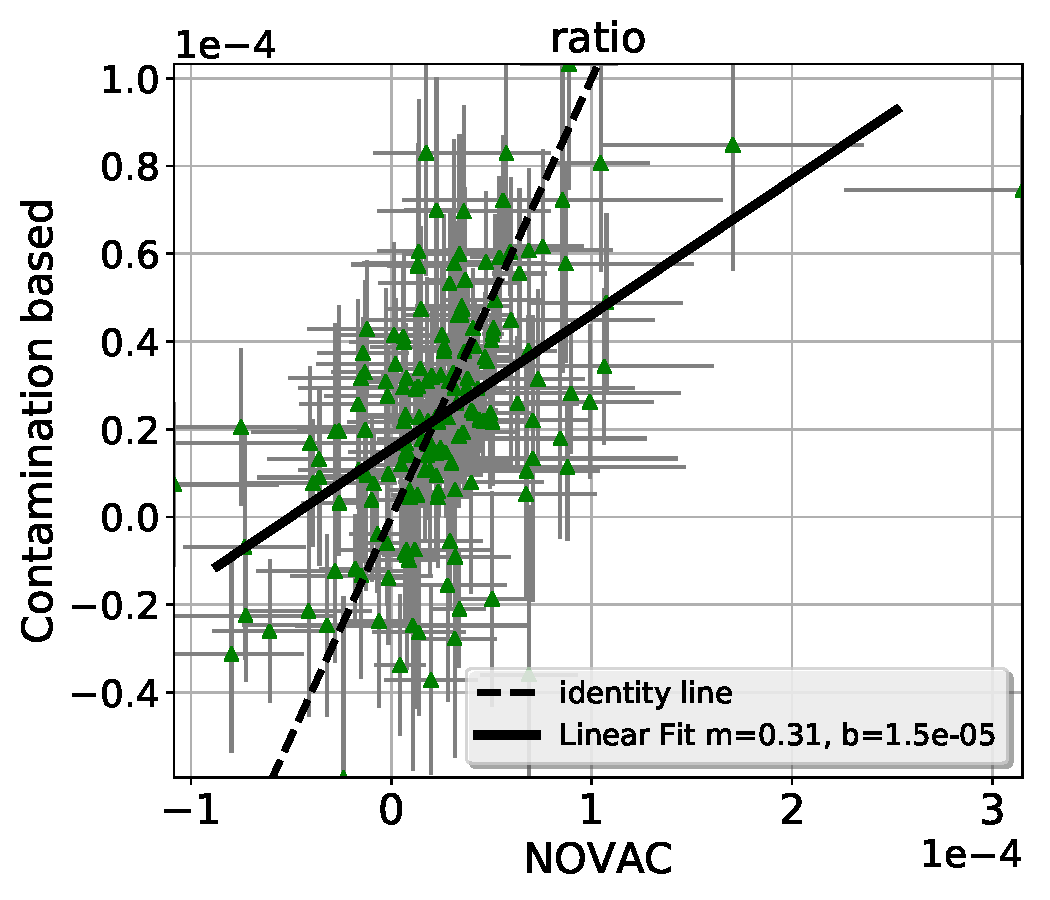
\includegraphics[width=0.49\textwidth]{../../Bilder/tung_ratio_novac_conbased}}
				\subfigure[Data of Nevado Del Riz]{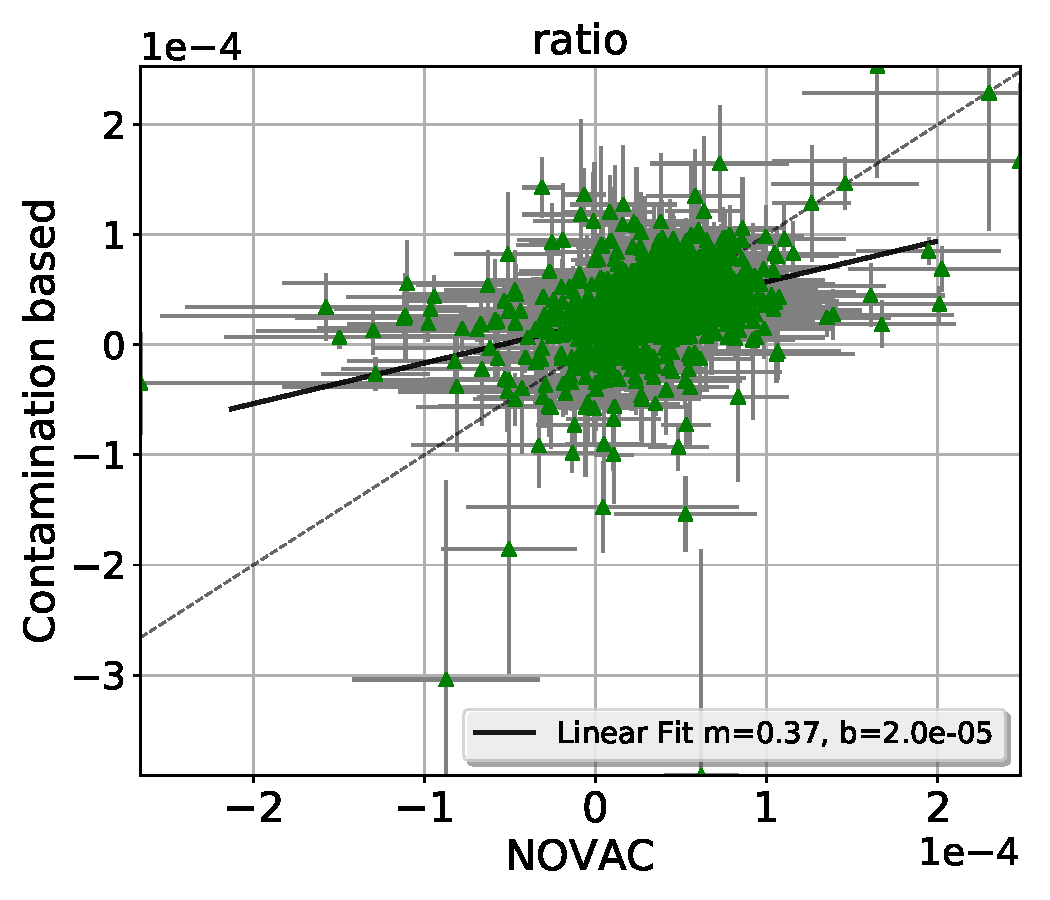
\includegraphics[width=0.49\textwidth]{../../Bilder/ratio_novac_conbased}}
			\end{figure}
			\begin{multicols}{2}
				\begin{itemize}
					\item Increase of low BrO/\ce{SO2} ratios
					\item Decrease of high BrO/\ce{SO2} ratios
				\end{itemize}
			\end{multicols}
		\end{frame}
		
		\begin{frame}
			\frametitle{\color{mygreen}Comparison with NOVAC evaluation\\%\rule{_Breite_}{_Stärke_} %%andersrum ist's vertikal;)
				\color{mygreen}{\rule{0.8\textwidth}{2pt}}}
			\begin{table}
				\begin{tabular}{p{3.5cm}p{2cm}p{3cm}}
					&Tungurahua&Nevado Del Ruiz\\
					\toprule
					Total Amount of Data&6500&14005\\
					\midrule
					Total amount of Data above Plume Limit&6.7\%&12.8\%\\
					\midrule
					Contaminated Data &6.0\%&9.9\%\\
					\bottomrule			
				\end{tabular}
			\end{table}
		\end{frame}
		
		\begin{frame}
			\frametitle{\color{mygreen}Comparison with NOVAC evaluation\\%\rule{_Breite_}{_Stärke_} %%andersrum ist's vertikal;)
				\color{mygreen}{\rule{0.8\textwidth}{2pt}}}
			\begin{table}
				
				\only<2>{		
					\begin{tabular}{p{2cm}p{2cm}p{2.5cm}p{2.5cm}}
						\multicolumn{4}{c}{\textbf{Contaminated data}}\\
						\toprule
						&&Tungurahua&Nevado Del Ruiz\\
						\toprule
						\multirow{2}{*}{\shortstack[l]{Within\\ Plume-limit}}& NOVAC&19.2\%&39.9\%\\
						&NEW&41.9\%&77.9\%\\
						\midrule
						not analysable&&2.5\%&7.8\%\\
						\bottomrule			
					\end{tabular}
				}
				\only<1>{	
					\begin{tabular}{p{2cm}p{2.5cm}p{3cm}}
						\multicolumn{3}{c}{\textbf{Not contaminated data}}\\
						\toprule
						&Tungurahua&Nevado Del Ruiz\\
						\toprule
						{\shortstack[l]{Within\\ Plume-limit}}&5.5\%&8.8\%\\
						
						\bottomrule		
					\end{tabular}}
				\end{table}
				\only<1>{\vspace{1cm}}
				\begin{itemize}
					\centering
					\only<2>{\item percentage refers to the contaminated data}
					\only<1>{\item percentage refers to the not contaminated data}
				\end{itemize}
				
			\end{frame}
			
			
			\begin{frame}
				\frametitle{\color{mygreen}Summary\\%\rule{_Breite_}{_Stärke_} %%andersrum ist's vertikal;)
					\color{mygreen}{\rule{0.8\textwidth}{2pt}}}
				
				\begin{itemize}
					\item Contaminated reference spectra lead to significant underestimation of SO$_2$ 
					\item Optimized Evaluation: Keep environmental conditions of measurement and reference spectra similar 
					
					\item More valid Data with optimized reference evaluation
					
				\end{itemize}
			\end{frame}
			\begin{frame}
				\frametitle{\color{mygreen}Outlook\\%\rule{_Breite_}{_Stärke_} %%andersrum ist's vertikal;)
					\color{mygreen}{\rule{0.8\textwidth}{2pt}}}
				
				\begin{enumerate}
					
					\item Measurements at volcanoes to verify the contamination
					\item Examine contamination of the plume due to further measurements
					\item Is contamination a result of low wind velocities? 
					
				\end{enumerate}
			\end{frame}
			
			
			
			
			
			\begin{frame}
				\thispagestyle{empty} % No slide header and footer
				\begin{tikzpicture}[remember picture,overlay] % Background box
				\node [xshift=\paperwidth/2,yshift=\paperheight/1.7] at (current page.south west)[rectangle,fill,inner sep=0pt,minimum width=\paperwidth,minimum height=\paperheight/2.5,top color=mygreen,bottom color=mygreen]{}; % Change the height of the box, its colors and position on the page here
				\end{tikzpicture}
				% Text within the box
				\begin{flushright}
					\vspace{1cm}
					\color{black}\sffamily
					{\bfseries\Large Thanks for your attention} % Title
					\vspace{0.8cm}
					\normalsize
					
					\vfill
				\end{flushright}
			\end{frame}
			
			
		\end{document}